En esta sección se presentarán los conceptos teóricos subyacentes en los que está basado este trabajo de investigación, que se utilizan a lo largo de este documento y son la base para comprender el marco en torno a él.

En la las primeras secciones, 2.1 a 2.6, se habla de las distintas estrategias, metodologías, y técnicas que envuelven el proceso de auditar un software. En las secciones 2.7 y 2.8 se introduce al compilador como un pilar importante en el proceso del desarrollo de software, y se explica su anatomía. Por último, en la secciones 2.9, 2.10 y 2.11, se presenta el concepto de una estructura blockchain, los smart contracts, y el lenguaje de interés Solidity, quién posee su propio compilador como parte del proceso de su utilización.


\section{Auditoría de software (seguridad)}
Uno de los \textit{aclamados} padres de la seguridad informática del software, comenzó preguntándose por qué los creadores de Java fallaron al aplicarle seguridad al lenguaje en su momento. Buscando sobre cómo aprender sobre ello, se descubrió para su sorpresa que hasta ese momento ningún libro se había escrito al respecto, siendo que se sitúa a mediados de los 90'.

Luego de eso, en el 2000 publicó un libro llamado \textbf{Building Secure Software} (construyendo software seguro), junto a John Viega, que terminó siendo el \textit{primer libro} en el mundo relacionado a seguridad en software.

Desde entonces se han publicado muchos otros libros\cite{McGraw:2006:SSB:1121680}\cite{Shostack:2014:TMD:2829295}\cite{Hoglund:2004:ESB:984253}\cite{Howard:2009:DSS:1594832}\cite{Klein:2011:BHD:2823924}\cite{Allen:2008:SSE:1386212}\cite{Wysopal:2006:ASS:1196390}\cite{Ransome:2013:CSS:2613389}, y se han aplicado estándares como \textbf{Building Security In Maturity Model}\cite{McGraw:2015:SSB:2675327.2675329} (BSIMM, al estilo CMMI que ahora es el estándar de facto para medir iniciativas de seguridad de software), así como también el \textbf{Estándar de Verificación en Seguridad de Aplicaciones}\cite{OWASP:AVSP} (ASVS de OWASP) y su versión abierta del \textbf{Software Assurance Maturity Model} (Modelo de Madurez de la Seguridad del Software) llamado \textbf{OpenSAMM}\cite{OWASP:OpenSAMM}.

Sin embargo, la mayoría de los artículos que se pueden encontrar relacionados acerca de la seguridad en software comienzan describiendo políticas robustas previo al desarrollo del producto, y desde allí avanzan implementando mejores prácticas y programación segura. El gran problema de ello es que no todos los sistemas que quieran incorporar seguridad hoy en día pueden aplicar esta estrategia, ya que por cuestiones de recursos, o incluso sentido común, no se justificaría comenzar el desarrollo íntegramente desde cero. Es por eso que soluciones como estas sólo tienden a evitar las vulnerabilidades y no tratar las posibles ya existentes, para proyectos que ya estén creados.

Si bien ha habido un gran incremento en la aplicación de seguridad a la hora de desarrollar un software, no existen muchos materiales que traten la búsqueda de vulnerabilidades.

\begin{notesBox}
\textbf{Vulnerabilidad de software versus bug}

Entendiendo el término bug como un error, equivocación, o descuidos en programas que resultan en comportamientos inesperados y no deseados, una vulnerabilidad es un bug con implicancias en seguridad, permitiendo a un atacante abusar de ella para obtener alguna especie de beneficio, ya sea conseguir accesos privilegiados, provocar la caída de un servicio, tomar el control de un sistema o adquirir información sensible. Utilizar esa falla para violar las políticas de seguridad de un proyecto es lo que se llama explotar una vulnerabilidad, y quién intenta explotarla es llamado atacante.
\end{notesBox}

\section{Auditando}
Auditar una aplicación es el proceso de analizar su código (en el formato de su fuente o binario) para descubrir vulnerabilidades que algunos atacantes podrían explotar. Realizando este proceso, se pueden identificar y cerrar agujeros de seguridad que de otra manera pondrían en un riesgo innecesario datos sensibles y recursos de negocios.

El contenido de la presente sección está desarrollado y profundizado en el libro \textit{The Art of Software Security Assessment: Identifying and Preventing Software Vulnerabilities}\cite{Dowd:2006:ASS:1196394} (El arte del asesoramiento de seguridad de software: Identificando y previniendo vulnerabilidades de software).

A continuación ejemplos de algunas situaciones que son de relevancia en las que se realiza una auditoría:\newline

\begin{tabular}{|p{4.3cm}|p{4.3cm}|p{4.3cm}|}
    \hline
    \textbf{Situación} & \textbf{Descripción} & \textbf{Ventaja} \\
    \hline
    Auditoría in-house (pre-release). & Una compañía de software realiza auditorías de código a un nuevo producto antes de su release. & Fallas de diseño e implementación pueden ser identificadas y remediadas antes de que el producto salga al mercado, ahorrando dinero en desarrollo y desplegando actualizaciones. También le ahorra a la compañía una potencial situación vergonzosa. \\
    \hline
    Aditoría in-house (post-release). & Una compañía de software realiza auditorías de código a un nuevo producto luego de su release. & 
    Vulnerabilidades de seguridad pueden ser encontradas y corregidas antes de que partes con intenciones maliciosas las descubran primero. Este proceso permite obtener tiempo para realizar testeos y otros chequeos, al contrario que estar haciendo una publicación en apuros en respuesta a un vulnerability disclosure (la acción de hacer pública una vulnerabilidad). \\
    \hline
    Comparación de productos por terceros. & Un tercero realiza auditorías a varios productos que compiten en un contexto dado. & Un tercero que pueda ser objetivo, puede proveer información útil a consumidores y asistirlos en seleccionar el producto más seguro. \\
    \hline
\end{tabular}
\pagebreak


\begin{tabular}{|p{4.3cm}|p{4.3cm}|p{4.3cm}|}
    \hline
    Evaluación por terceros & Un tercero realiza una auditoría de software de manera independiente para un producto de un cliente. & El cliente puede obtener un gran entendimiento de la seguridad relativa a un producto que pretende desplegar. Esto prueba ser el factor decisivo entre la compra de un producto u otro. \\
    \hline
    Evaluación preliminar por terceros. & Un tercero realiza una auditoría de software de manera independiente de un producto antes de que salga al mercado. & Capitalistas de riesgo pueden obtener una idea de la viabilidad de una futura tecnología con propósitos de financiamiento. Proveedores pueden también realizar este tipo de evaluación para asegurar la calidad de un producto que pretenden llevar al mercado. \\
    \hline
    Investigación independiente. & Una compañía de seguridad o una firma de consultoría realiza una auditoría de software de manera independiente. & Proveedores de productos de seguridad pueden identificar vulnerabilidades e implementar medidas de protección en scanners y otros dispositivos de seguridad. La investigación independiente también funciona como una industria que está atenta y provee una manera para que los investigadores y compañías de seguridad establezcan credibilidad profesional. \\
    \hline
\end{tabular}

\subsection{Auditando versus black box testing}
La idea del black box, o testeo de caja negra, es evaluar un sistema solamente manipulando sus interfaces, en el cual la estructura, el diseño o la implementación interna del objeto que se está analizando no es conocido por el profesional de validación (tester). Es llamado así, porque el software a ojos del tester es como una caja en la cual el contenido no se puede ver.

Desde la perspectiva de seguridad, y no tanto asociado a las definiciones formales, como la que podría proveer a los profesionales informáticos el \textbf{International Software Testing Qualifications Board} (Comité Internacional de Certificaciones de Pruebas de Software), lo que se busca es comunicarse con estas interfaces de maneras inesperadas para la lógica contenida en el software. Es decir, si se está testeando con esta metodología un servidor web (web server), se enviarán variantes de peticiones de protocolo \textbf{HTTP} (Hyper Text Transfer Protocol) reales, malformadas, e incluso modificadas para ser de un tamaño mayor al posiblemente esperado.

Cualquier comportamiento inesperado, o el mero detenimiento del software analizado es considerado algo de gran seriedad. El hecho de automatizar este proceso, para acelerar el hallazgo de más fallas, es llamado \textbf{\textit{fuzz-testing}}, del cual se hablará con profundidad más adelante.

A menudo, analizando código manualmente se pueden encontrar vulnerabilidades que realizando tareas automatizadas probablemente pasen por alto, y es por eso que existe la necesidad de realizar asesoramientos a las estructuras del código de manera inteligente, en adición a simplemente correr herramientas automatizadas observando sus resultados. Es necesario poder analizar código, y detectar caminos y/o vulnerabilidades que una herramienta puede llegar a pasar de largo.

Afortunadamente, la combinación de auditar manualmente y el uso de black box testing provee una combinación útil en cortos plazos de tiempo.
\subsection{Auditoría de código y el ciclo de desarrollo de software}
Cuando se consideran los riesgos de exponer una aplicación a potenciales usuarios maliciosos, el valor de un asesoramiento de seguridad está claro. Sin embargo, hay que saber exactamente cuándo realizarlo. Generalmente se puede realizar una auditoría en cualquier momento del ciclo vital del desarrollo/diseño de sistemas\cite{Highsmith2001AgileSD} (Systems Development Life Cycle, de ahora en más \textbf{SDLC}), pero el costo de identificar y corregir las vulnerabilidades encontradas no va a ser lo mismo para cualquier etapa de él. 

Según la opinión del autor, los desarrolladores parecen pasar su vida entera encerrados en el SDLC, no importa si utilizan métodos ágiles, DevOPs, cascada, etc., siempre hay un análisis, una etapa de diseño, otra de implementación o código, y otra de testing (no siempre presente). Finalmente existe por lo general una etapa de operaciones, donde hay monitoreo.

Desde el punto de vista profesional, se observa una diferencia destacable entre lo que se conoce como un desarrollador puro y un ingeniero de sistemas. La diferencia reside en que los primeros, simplemente desarrollan piezas de software por lo general, sin seguir un proceso (o siguiéndolo sin necesidad de comprenderlo profundamente), mientras que los últimos están capacitados para diseñar y aplicar procesos, incluyendo también seguridad en ellos.

En relación de cómo la seguridad afecta al SDLC se puede decir lo siguiente\cite{GaryMcGrawSoftwareSecurity}\cite{TheSDLCMicrosoft}\cite{SoftwarePenetrationTesting}\cite{Manicode:SSDLC}:
\begin{itemize}
\item \textbf{La seguridad es invasiva.} \newline Si un desarrollador hoy en día no está de manera rigurosa involucrando la seguridad en su código, cuando ésta aparezca, que inevitablemente lo hará, lo sentirá invasivo, ya que deberán hacerse muchos cambios, y por naturaleza el humano es resistente al cambio (hay una gran rama de investigación bajo el acrónimo RTC que explica muy bien esta temática).
\item \textbf{La seguridad no puede ser aplicada como un parche al final del proyecto.} \newline \textit{Gary McGraw}, previamente mencionado, y uno de los padres de la seguridad de la seguridad informática, comenzó siempre diciendo que la seguridad debe construirse en conjunto con el software, no agregarlo como algo después.
\item \textbf{El sistema debe ser desarrollado con la seguridad activa por defecto.} \newline El término \textbf{security by default} (seguro/seguridad por defecto) proviene de proveer un sistema o software, con la configuración más segura que se puede obtener por defecto. Esto no hace que el software sea impenetrable, sino que ahorra a los usuarios el tener que estar pendientes de una configuración para prevenirse, cuando puede que realizarla sea de una complejidad relevante.
\item \textbf{El software debe ser escrito de manera segura desde el comienzo.} \newline En el proceso hay que darle a la seguridad una alta prioridad, como aspectos claves del núcleo del proyecto, no como \textit{features} (características adicionales) que van a ser agregados luego. Conviene atender estos aspectos desde el comienzo. 
\item \textbf{No subestimar la resistencia del equipo de desarrollo.} \newline No subestimar la resistencia de los desarrolladores, ya que el hecho de tener que implementar seguridad en los sistemas hace que se incremente la complejidad y se retrase el tiempo para alcanzar la funcionalidad. El autor opina desde su experiencia que los desarrolladores en la industria están acostumbrados a que les paguen por cosas que funcionen.
\item \textbf{Una relación cercana con el experto adecuado y la unidad de gestión desde el principio es un requerimiento que no debe ser negociado.}
\end{itemize}

Todo proceso de desarrollo de software sigue este modelo hasta cierto grado. El clásico modelo en cascada tiende a moverse hacia una interpretación estricta, en donde el tiempo de vida del sistema solamente itera una sola vez sobre el modelo. En contraste, nuevas metodologías, como desarrollo ágil\cite{ries2012metodo}, tienden a enfocarse en refinar la aplicación realizando repetidas iteraciones de las fases del SDLC. Entonces la forma en la que el modelo SDLC se aplica puede variar, pero los conceptos básicos y las fases son lo suficientemente consistentes para los propósitos de esta discusión.

\begin{figure}[h]
    \centering
    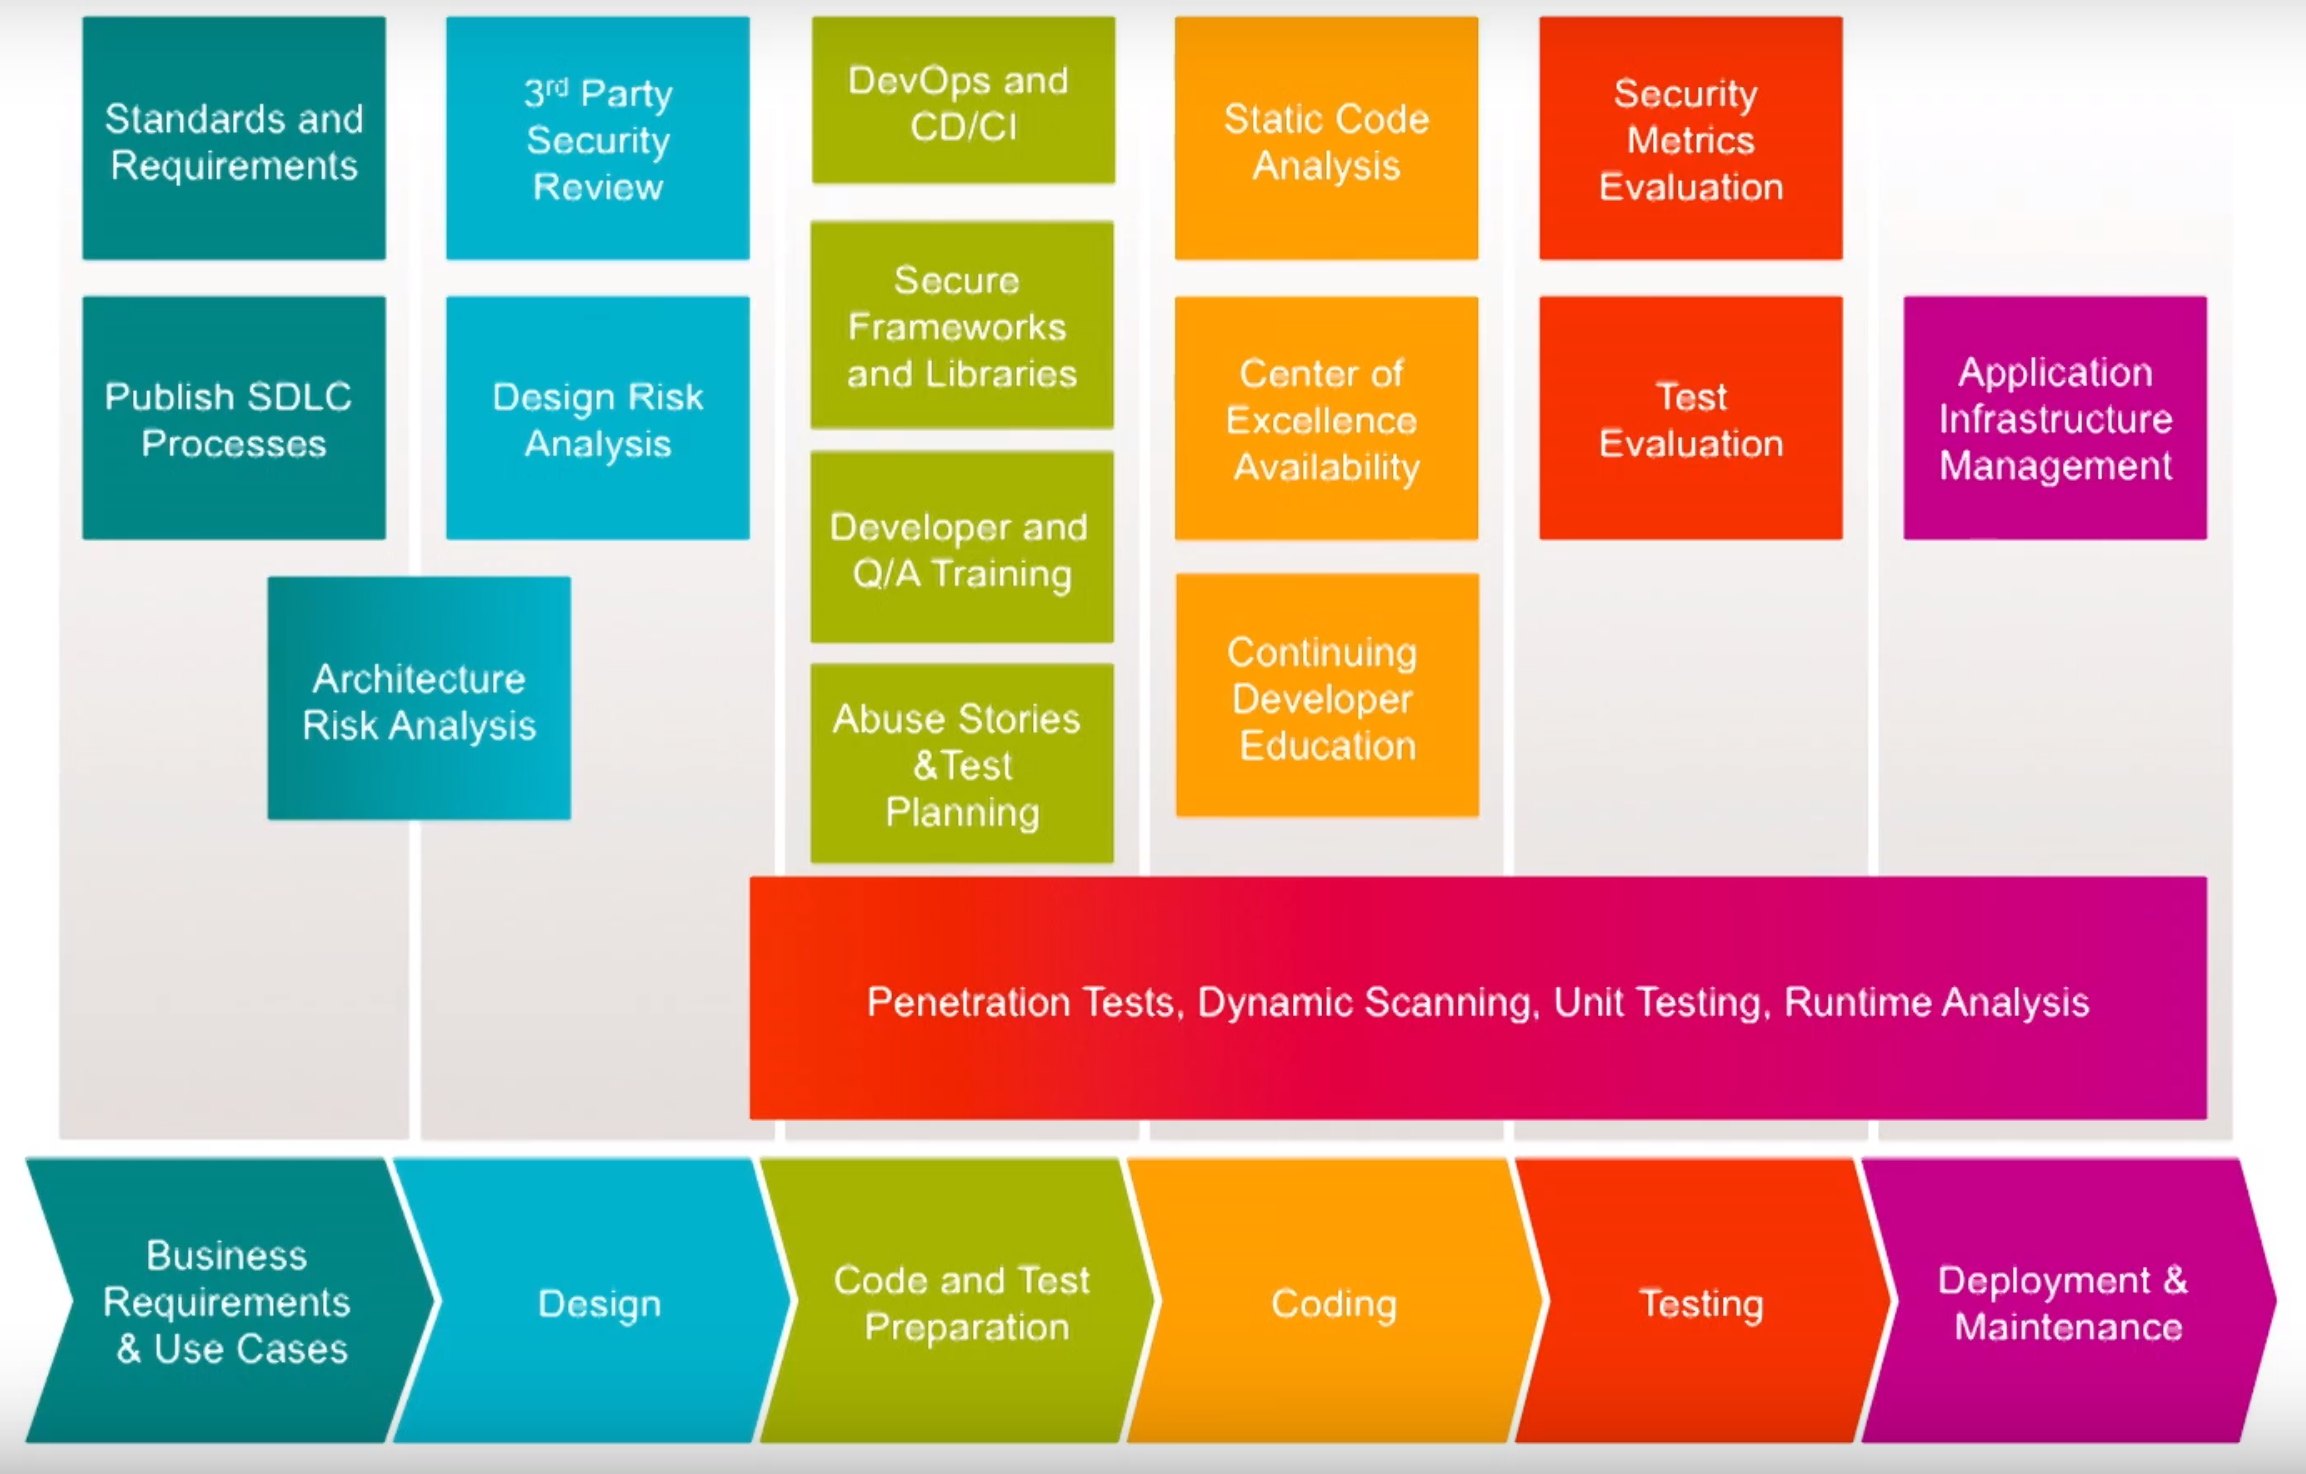
\includegraphics[scale=0.19]{images/JimManicodeSSDLC.png}
    \caption{Security in the SDLC, Jim Manico, dotSecurity 2017.}
    \label{fig:ssdlc}
\end{figure}

Entendiendo que aplicar seguridad en distintas etapas del proceso puede llevar a hallazgos en cada una de ellas, es natural poder separar en categorías cada uno de estos hallazgos. Para ver una representación de cómo sería ver la Figura \ref{fig:ssdlc}.
Si lo que se encuentra corresponde a la etapa de diseño, tienden a ser fallas en las especificaciones y la arquitectura del sistema; vulnerabilidades de implementación son fallas técnicas a bajo nivel en la construcción real del software, y finalmente, en la categoría de vulnerabilidades operacionales  entran las fallas que suceden por deployments y configuración del software en un entorno en particular.

Sin ir más lejos, los costos para solucionar un bug en algunas de estas etapas, tanto para proyectos ágiles o en cascada, empeoran mientras más tarde se encuentran.

A continuación se mencionan algunos hechos relevantes y destacados por su impacto, relacionados a bugs de fallas de seguridad. 
El Mariner 1 de la NASA fue el primer intento de Estados Unidos de enviar una nave espacial a Venus. Poco después de su lanzamiento en 1962, se desvió del rumbo debido a un error de software. Un empleado de la \textbf{NASA} se vio obligado a mandar a la nave a autodestruirse. Se quemaron \$ 18 millones de dólares debido a un guión (-) faltante en el código\cite{TrueCostSoftBugCelerity}.

En febrero del 2018 los servicios web de \textbf{Amazon} no estuvieron disponibles durante 4 horas y afectaron a innumerables sitios. Aunque el costo financiero no está claro, las estimaciones de cuando el sitio de Amazon se cayó en 2016 durante 20 minutos fue de \$ 3.75 millones. El incidente de este verano fue 12 veces más largo e involucró a muchos otros sitios web.

\textbf{AT\&T} actualizó su software para llamadas de larga distancia en enero de 1990. Sin embargo, no se percataron de que el sistema no podría mantenerse al día con la velocidad del nuevo programa. Las llamadas de larga distancia cayeron durante 9 horas. Se perdieron 200,000 reservas de aerolíneas y hubo 75 millones de llamadas telefónicas perdidas. El costo total estimado para AT\&T fue de \$ 60 millones \cite{TrueCostSoftBugCBT}.

El Instituto de Ciencias de Sistemas de \textbf{IBM} ha informado que \textit{el costo de reparar un error después de la publicación del producto fue de cuatro a cinco veces más que uno descubierto durante el diseño, y hasta 100 veces más que uno identificado en la fase de mantenimiento.}


\subsection{Costos en el tiempo}
Phil Crosby, autor que contribuyó a las prácticas de la gestión de la calidad, en su libro \textbf{Quality is free} (La calidad es gratis) explica cuánto cuesta la mala calidad a largo plazo en un proyecto. Simplificadamente se puede interpretar en el gráfico de la Figura \ref{fig:cost of a defect}. El cual intenta demostrar que mientras más temprano, y en etapas más internas se puedan localizar los problemas, más económico será el costo/tiempo de resolverlos, ya que se involucrará menos gente en el proceso.

\begin{figure}[h]
    \centering
    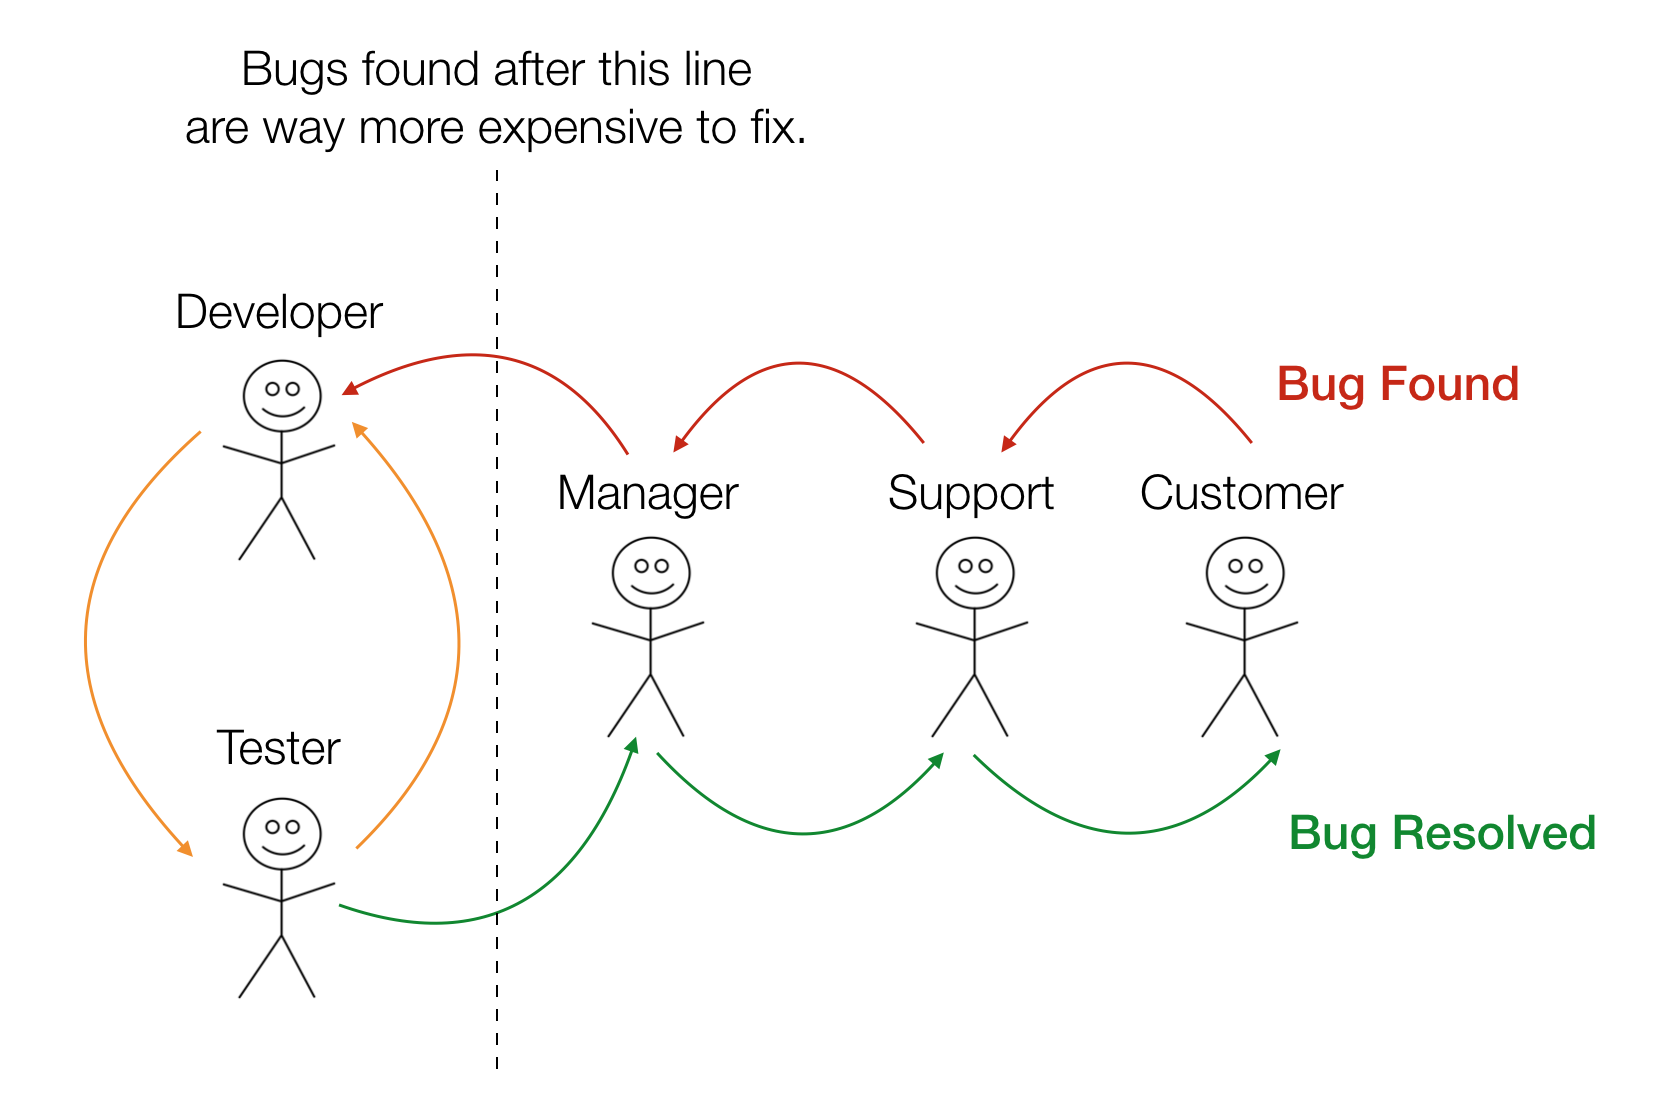
\includegraphics[scale=0.5]{images/the_cost_of_a_defect.png}
    \caption{Cost of a software bug, Emanuil Slavov.}
    \label{fig:cost of a defect}
\end{figure}

Para un ciclo de desarrollo en cascada, según Caper Jones, especialista en metodologías de ingeniería de software, y asociado con el modelo de punto de función de estimación de costos, en su libro Applied Software Measurement: Assuring Productivity and Quality\cite{jones2008applied} el costo para corregir un bug en las distintas etapas se ve descrito por el gráfico de la Figura \ref{fig:applied cost measurement}

\begin{figure}[h]
    \centering
    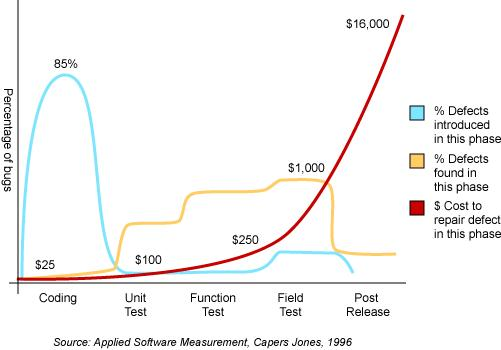
\includegraphics[scale=0.5]{images/AppliedSoftwareMeasurement.png}
    \caption{Applied Software Measurement, Caper Jones, 1996.}
    \label{fig:applied cost measurement}
\end{figure}

Steve McConnell autor de muchos libros de texto de ingeniería de software conocidos, como \textbf{Code Complete}\cite{mcconnell2004code}, \textbf{Rapid Development}\cite{mcconnell1996rapid}, y \textbf{Software Estimation}\cite{mcconnell2006software}, en su primero también realiza un análisis en la dirección de Caper Jones. En la Figura \ref{fig:defect cost increase}, de uno de sus libros se puede observar el costo de detectar un defecto en determinadas etapas.

\begin{figure}[h]
    \centering
    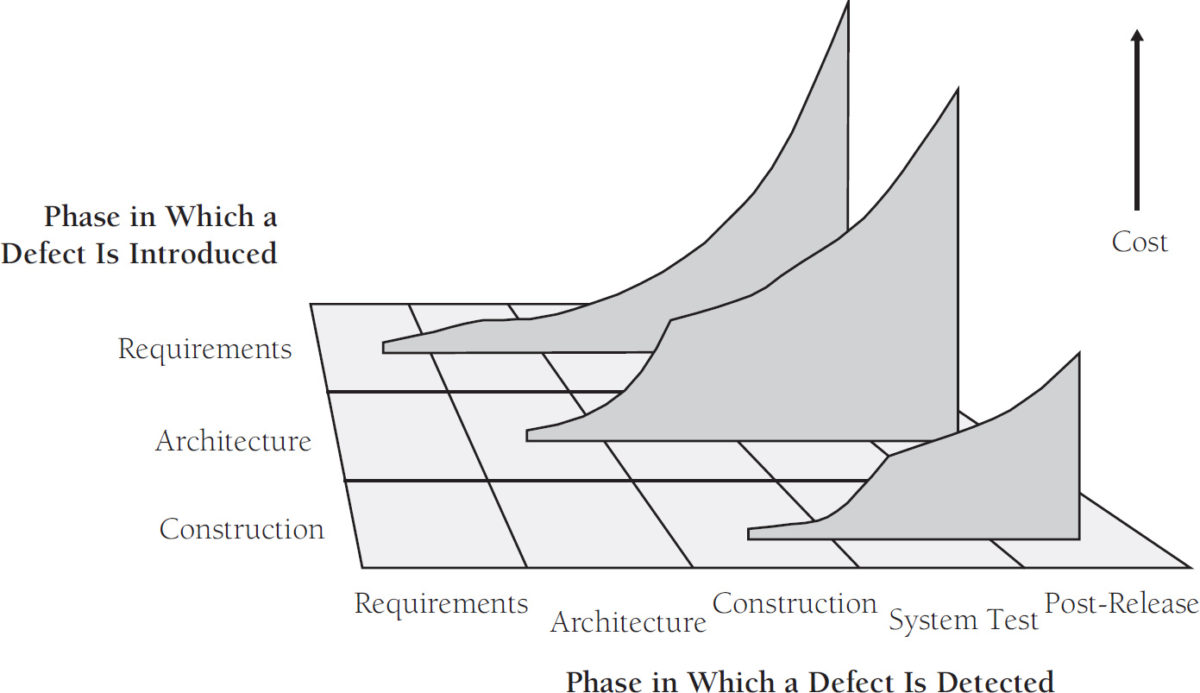
\includegraphics[scale=0.3]{images/DefectCostIncrease2004.jpg}
    \caption{Costo de encontrar defectos por fase, Steve McConnell en Code Complete, 2004.}
    \label{fig:defect cost increase}
\end{figure}

En la Figura \ref{fig:cost-of-change curve} se encuentra una visualización de un artículo sumamente detallado, llamado The Agile Difference for SCM\cite{TheAgileDifference} (La diferencia ágil para la administración de la cadena de suministro), comparando los costos para los distintos modelos: XP, Boehm y Ágil.

\begin{figure}[h]
    \centering
    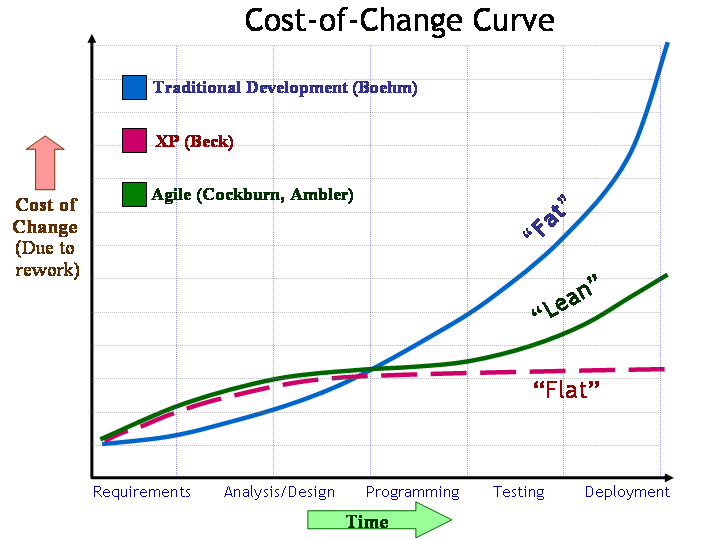
\includegraphics[scale=0.5]{images/TheAgileDifference.png}
    \caption{Curvas del costo de un cambio, CM Crossroads.}
    \label{fig:cost-of-change curve}
\end{figure}

Scott W. Ambler un ingeniero de software, consultor, autor de varios libros centrados en el kit de herramientas de Disciplined Agile Delivery, el proceso Unificado, el desarrollo de software Agile, el Lenguaje de modelado unificado y el desarrollo del Modelo de madurez de capacidades. En su publicación \textbf{Why Agile Software Development Techniques Work: Improved Feedback}\cite{ambler2006agile} (Por qué las técnicas ágiles de desarrollo de software funcionan: Feedback mejorado) se puede observar otro gráfico en relación a los costos con respecto a lo avanzado que se está en el desarrollo del proyecto:

\begin{figure}[h]
    \centering
    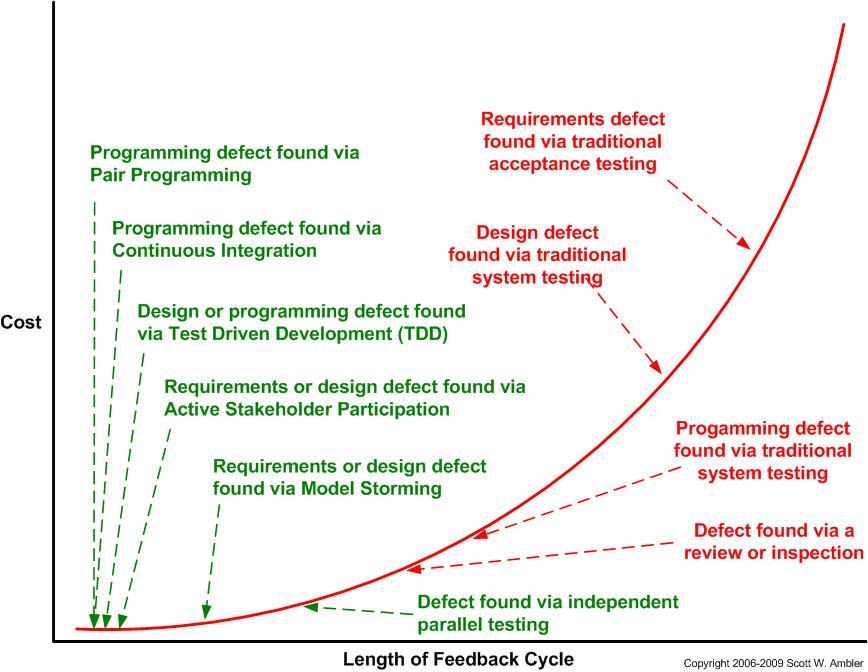
\includegraphics[scale=0.5]{images/ComparingTechniques.jpg}
    \caption{Longitud y costo de un defecto dentro del ciclo de desarrollo, Scott W. Ambler}
    \label{fig:cost-of-change curve}
\end{figure}

A esta altura se puede asumir que el lector tiene una interpretación, al menos visual, respaldada de distintas fuentes con años de trayectoria de lo que cuesta posponer la búsqueda de problemas y solucionarlos en etapas tempranas.

Ahora, hay que entender que estos estudios no contemplan errores de seguridad, ya que tienden a ser superiores, porque si son vulnerabilidades explotables, tienen un impacto directo y dañino, en la empresa y sus consumidores; los impactos directos de reputación también no fueron cuantificados en los estudios anteriores.

Las violaciones a la seguridad cuestan al rededor 600 mil millones de dólares al año globalmente\cite{mcafeecsis}. El 46\% de los incidentes de ciberseguridad del 2017 son debidos a personas internas a la organización\cite{kasperskyHumanFactor}. El 30\% de los profesionales de seguridad esperan un gran y efectivo ataque dentro de los próximos 90 días.\cite{theeconomistCyberChasm}

La mayoría de las fallas en los mecanismos de seguridad están relacionadas a funcionalidad faltante o incorrecta, y la mayoría de las vulnerabilidades están relacionadas a comportamientos adversos no intencionales. 

Michael Felderer, et. al., explican muy bien en su sección de Security Testing\cite{FELDERER20161} en Advances in Computers, 2016:
Las pruebas (funcionales) normalmente se centran en la presencia de algún comportamiento correcto, pero no en la ausencia de un comportamiento adicional, que está implícitamente especificado por requisitos negativos. Las pruebas rutinariamente omiten las acciones ocultas y el resultado son comportamientos peligrosos de efectos secundarios que se envían con un software. La Figura \ref{fig:functionality side-effects} siguiente ilustra esta naturaleza de efectos secundarios de la mayoría de las vulnerabilidades de software que las pruebas de seguridad tienen que enfrentar\cite{FELDERER20161}.

\begin{figure}[h]
    \centering
    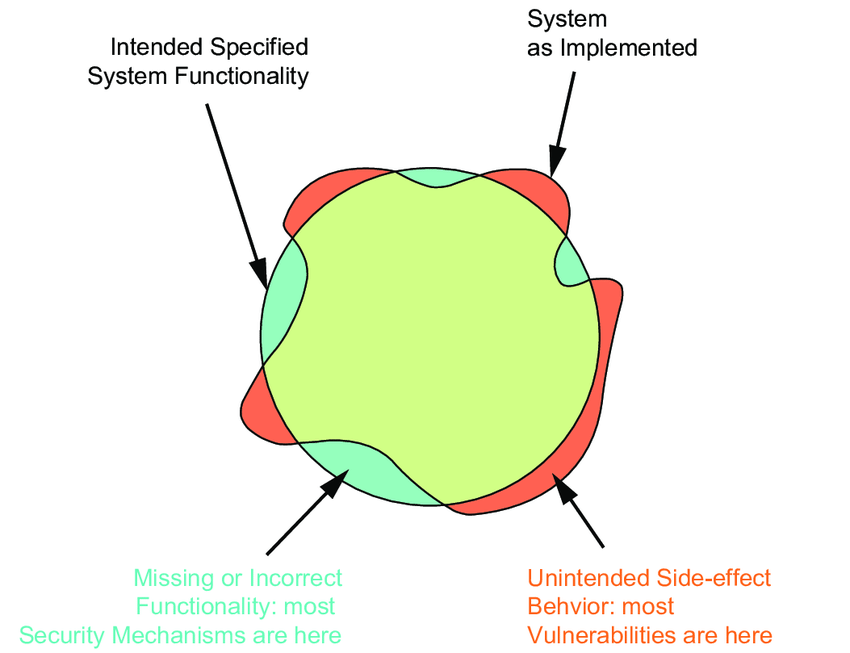
\includegraphics[scale=0.5]{images/functionality.png}
    \caption{Security Testing: A Survey, Michael Felderer.}
    \label{fig:functionality side-effects}
\end{figure}

El círculo representa la funcionalidad prevista de una aplicación, incluidos los mecanismos de seguridad, que generalmente se define mediante la especificación de requisitos. La forma amorfa superpuesta en el círculo representa la funcionalidad real e implementada de la aplicación. En un sistema ideal, la aplicación codificada se superpondría completamente con su especificación, pero en la práctica, este casi nunca es el caso. Las áreas del círculo que la aplicación codificada no cubre representan fallas funcionales típicas (es decir, comportamiento que se implementó incorrectamente y no se ajusta a la especificación), especialmente también en los mecanismos de seguridad. Las áreas que quedan fuera de la región circular representan una funcionalidad no intencionada y potencialmente peligrosa, donde residen la mayoría de las vulnerabilidades de seguridad. La falta de coincidencia entre la especificación y la implementación que se muestra en la figura que conduce a fallas en los mecanismos de seguridad y vulnerabilidades se puede reducir teniendo en cuenta los aspectos de seguridad y especialmente las pruebas de seguridad en una etapa temprana y en todas las fases del ciclo de vida del desarrollo de software.

Dentro de la misma investigación, y basándose de manera abstracta a partir de técnicas de prueba de seguridad concretas mencionadas anteriormente, se clasifican en la siguiente figura de acuerdo con su base de prueba dentro del SSDLC.

\begin{figure}[h]
    \centering
    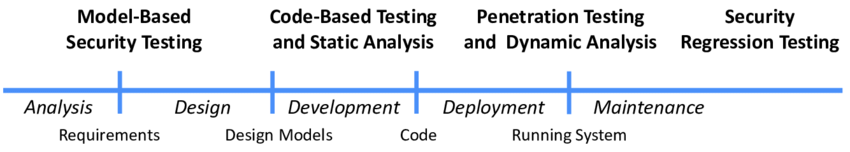
\includegraphics[scale=0.5]{images/TechniquesInTheSSDLC.png}
    \caption{Técnicas de prueba de seguridad en el ciclo de vida de desarrollo de software seguro.}
    \label{fig:ssdlc techniques}
\end{figure}

Las pruebas de \textit{seguridad basadas en modelos} se basan en requisitos y modelos de diseño creados durante la fase de análisis y diseño. Las \textit{pruebas basadas en código y el análisis estático} se basan en el código fuente y el bytecode creado durante el desarrollo. Las \textit{pruebas de penetración y el análisis dinámico} se basan en sistemas en ejecución, ya sea en un entorno de prueba o de producción. Finalmente, las \textit{pruebas de regresión de seguridad} se realizan durante el mantenimiento.


\section{Proceso de revisión de software}
Cuando se tiene que comenzar con el proceso de revisar, desde la perspectiva de seguridad, un software que jamás se ha visto, teniendo una ventana de tiempo generalmente acotada, hay que entender cómo utilizar los recursos y poder cubrir bien las partes que son más relevantes a la seguridad.

Adoptando un proceso pragmático, flexible y basado en resultados se podrá obtener un balance para descubrir fallas de diseño, lógicas, operacionales y de implementación.

Hay dos frases que se destacan mucho de uno de los libros más importantes que he el autor ha tenido la oportunidad de leer en esta investigación, y son \textit{"la revisión de código es un proceso fundamentalmente creativo"}, y \textit{"hacer revisión de código es una habilidad"}. 

Entendiendo esto entonces, la mejor manera de realizarlo es armando una lista de todo lo que probablemente pueda salir mal, y al hacer la revisión tratar de entender al desarrollador pensando en situaciones que no haya podido anticipar. Es una especie de estudio del perfil (profiling) del equipo de desarrollo, y entender que no sólo pueden tener fallas a nivel código sino también conceptuales que en el mismo proyecto pueden traer consecuencias a la forma de encarar otras partes del mismo proyecto, o futuros. Por ejemplo, puede que para un \textit{input} (entrada) de usuario no se estén realizando los chequeos necesarios pero que no tenga ningún impacto real de seguridad; lo que no significa que en otros lugares del mismo proyecto esté aplicado de una forma diferente, pudiendo así explotar finalmente la falla, ya que ha sido conceptual o de diseño.

Tener un proceso es algo realmente valioso más allá de que hay más factores involucrados que simplemente seguir unos pasos. No todos los que realicen el mismo proceso obtendrán los mismos resultados, pero sí probablemente los haga más efectivos. Un proceso le da estructura a la auditoría, permite mantener un nivel de prioridades y ser consistente en el análisis. También de esta manera, junto con documentación permite que los asesoramientos sean algo compatible desde la perspectiva de negocios, lo cual no es algo menor, y es poco común.

El proceso de revisión que se mencionará a continuación, del cual hablan Mark Dowd, John McDonald, y Justin Schuhes, sobre la \textit{identificación y prevención de vulnerabilidades de software}, es abierto, adaptable a los requerimientos de cada equipo para prácticas reales, y está dividido en 4 etapas:
\begin{itemize}
\item \textbf{Pre asesoramiento:} recolección de información inicial y documentación; planeamiento y alcance de la auditoría.
\item \textbf{Revisión:} fase principal del asesoramiento. No está necesariamente estructurada en distintas etapas del ciclo de desarrollo. De hecho, estas etapas son objetivos simultáneos alcanzados por el uso de distintas estrategias. 
\item \textbf{Documentación y análisis:} documentación de procesos, hallazgos, y análisis sobre los mismos para evaluar riesgos y posibles métodos de solución. 
\item \textbf{Reporte y soporte de soluciones:} esta fase es básicamente para darle un seguimiento a quienes van a actuar en base a los hallazgos reportados.
\end{itemize}

\subsection{Pre asesoramiento}
En esta etapa se trata de obtener la mayor cantidad de información posible, porque a partir de ella se va a dictaminar cómo comenzar y qué acercamiento tomar frente a la auditoría.

Hay que definir bien el alcance del proyecto, tal vez sea buscar la vulnerabilidad más impactante del proyecto como también obtener la mayor cobertura del código posible sin la necesidad de comprobar que sean explotables o no las fallas encontradas. Esto no sólo va a depender de quién esté realizando la auditoría sino también del propósito de la misma.

Como forma tangible del software en cuestión se puede proveer tanto el código, como el binario, o ambos. La combinación del código y el binario, o un setup en el cual desde el código se pueda llegar al binario, son lo que hacen una revisión más eficiente (no siempre se puede llegar del código a un ejecutable). Sin un binario, ni la posibilidad de compilar, generalmente se realizan análisis estáticos, y en las potenciales fallas encontradas resultan difíciles de comprobar su real explotación. Sin el código fuente, no hay otra alternativa que realizar análisis en ejecución e ingeniería inversa (analizar el código assembler del ejecutable).

Existen otras alternativas, como poseer el binario con información adicional de debugging (símbolos por ejemplo) que facilita la ingeniería inversa, usualmente entregado por empresas con software propietario que quieren simplificar la revisión. Y el caso más extremo, usualmente más utilizado al realizar auditorías web, es cuando no se entrega código ni binario, en donde sólo se realizan técnicas externas como \textit{black box} y \textit{fuzzing} (*).

\textit{Fuzzing} es una forma de descubrir errores en el software al proporcionar entradas aleatorias a programas para encontrar casos de prueba que causan un \textit{crash} (detenimiento abrupto). Aplicando técnicas de \textit{fuzzing} a programas, se puede obtener una vista rápida de la solidez general y ayudar a encontrar y corregir errores críticos. Es una técnica de \textit{black box}, que no requiere acceso al código fuente, pero aún puede usarse contra el software para el que se posee dicho fuente, ya que posiblemente encuentre los errores más rápido, evitando la necesidad de revisar muchas líneas de código. Una vez que se detecta un bloqueo, si se tiene el código fuente, debería ser mucho más fácil de solucionar o explotar una vulnerabilidad.

En el caso de proyectos open source, como el que se verá en el caso de estudio, es donde se posee el mejor escenario. Para estos, siempre es mejor realizar una revisión manual de código, y como tal se debe comenzar con un \textit{threat model} (modelado de amenazas) o al menos entrevistas a los desarrolladores para tener un entendimiento de la arquitectura de la aplicación, su superficie de ataque, así como también las técnicas de implementación.

\subsection{Revisión}
La tendencia principal a la hora de comenzar es generalmente seguir un modelo en cascada, lo cual no siempre es el mejor camino o el único, como ya se ha hablado anteriormente, más si se está hablando en términos de ser tiempo-eficiente identificando vulnerabilidades en alto como bajo nivel.
Parecerá obvio pero un auditor se encuentra más preparado para juzgar la seguridad del diseño o implementación, al finalizar la auditoría que al principio. Esto es, hablando en términos de entenderlo de manera abstracta.

No siempre se puede comenzar por el diseño o haciendo un \textit{threat model}, a veces la documentación no existe, está incompleta, vieja; los desarrolladores pueden también no estar disponibles.

El método para realizar la revisión es un simple proceso iterativo. Particularmente se planea qué estrategia utilizar, y dependiendo de ella la selección de técnicas u objetivos. Después se ejecuta la estrategia seleccionada tomando notas, y de vez en cuando reflexionar sobre el manejo del tiempo, para no obsesionarse particularmente con algo que demande demasiado. Finalmente entender qué es lo que se ha aprendido y ver cómo utilizarlo, repitiendo estos pasos hasta el final de la auditoría.

Hay tres maneras generalizadas para realizar la evaluación: \textit{top-down}, \textit{bottom-up}, e híbrida; las primeras dos son análogas a los tipos de descomposición de componentes en el diseño de software, y la última una combinación de ambas, alternando, dependiendo cuanta información se tenga del contexto dado.

En la etapa de planeamiento se elige qué tipo de estrategia se utilizará, en las próximas secciones se detalla brevemente las recomendadas por estos autores. La selección, la preparación para la misma y demás detalles se realizan dependiendo si se trabaja en equipo, con metas/objetivos específicos, y preparación de la toma de notas/documentación que se va a acontecer. También se pone sobre la mesa hacer un chequeo general del estado de la evaluación, re-evaluar si la estrategia seleccionada está funcionando, y conducir \textit{peer-reviews} para tener más objetividad.

\subsection{Documentación y análisis}
En esta etapa, luego de que el trabajo difícil ha terminado, se documentan o formalizan las notas que se tomaron con los hallazgos. 

Principalmente se puede describir el tipo de amenaza, el componente afectado, el módulo (línea de código) donde se encontró, a qué clase de vulnerabilidad pertenece, una descripción con el resultado y el contexto para reproducirla. Finalmente el riesgo o impacto que produce.

Se decidió no entrar en detalles en cómo es cada una de las categorías ya que son bastante explicativas por sí solas, y depende de la dedicación que se le quiera abocar a cada una, tanto como agregar mas o utilizar menos.

\subsection{Reporte y soporte de soluciones}
Finalizar una auditoría no consta solamente de entregar lo hallado de manera organizada. Se cumple un rol muy importante a la hora de entregar, ya que sin alternativas, soluciones o sin mantener un contacto para ayudar a remediar los problemas reportados nos estaría faltando una parte muy importante de nuestro trabajo.

Dependiendo del tipo de auditoría que se esté realizando, esta etapa puede implicar situaciones más complejas. En caso de una investigación independiente, en la circunstancia de haber encontrado vulnerabilidades explotables que pueden perjudicar a otros usuarios, se debe iniciar un disclosure (divulgación) responsable. Generalmente se desarrollan exploits (programa particularmente diseñado y/o utilizado para abusar vulnerabilidades en un determinado sistema) antes de contactar al proveedor de ese software/servicio, y una vez contactado, en el caso de respuesta, se otorgan 30-90 días para solucionar el problema antes de hacerlo público.

\begin{notesBox}
    \textbf{Recorrer el código}
    Al autor le parece importante dejar expresado brevemente la importancia que tiene saber recorrer un código, porque es lo que se va a estar haciendo la mayor parte del tiempo, y dependiendo de la manera en la que se haga va a condicionar la velocidad y dificultad de su progreso.

    Generalmente, lo que es más efectivo es revisar funciones de manera aislada, y hacer seguimiento al flujo sólo cuando es absolutamente necesario.

\end{notesBox}

\section{Estrategias de auditoría de código}
Las estrategias se pueden resumir a las siguientes tres categorías:

\subsection{Compresión de código (CC):}
Estas estrategias analizan el código directamente para descubrir vulnerabilidades y mejorar el entendimiento de la aplicación.

En esta categoría se encuentran las siguientes metodologías: seguimiento de \textit{inputs} maliciosos, analizar un módulo, analizar un algoritmo, analizar una clase u objeto y seguimiento de cosas de interés por usar \textit{black box}.

Exceptuando por el seguimiento a los resultados encontrados realizando \textit{black box}, todas ellas son difíciles y lentas, pero todas las comprensiones de los impactos hallados serán altísimas.

\subsection{Puntos candidatos (CP):}
Se requieren dos pasos: Primero crear una lista de problemas potenciales mediante un proceso o mecanismo y luego examinar el código en busca de ellos.

En la lista mencionada se encuentran las siguientes estrategias: herramientas automatizadas de análisis del código; puntos candidatos de enfoque general, léxicos simples, binarios simples, generados por \textit{black box}, y específicos de aplicación. Estas estrategias se destacan por ser rápidas, fáciles de realizar pero la comprensión de su impacto suele ser bajo.

\subsection{Generalización de diseño (DG):}
Estas técnicas, son más flexibles, intencionadas para analizar potenciales problemas de medianos a alto nivel en la lógica y el diseño.

En ella se encuentran las siguientes sub-estrategias: modelado del sistema, testeo de hipótesis, deduciendo propósito y funcionalidad, y chequeo de conformidad de diseño.

Son de nivel moderado a difícil, velocidad media, pero con altísima comprensión del impacto.

\section{Tácticas de auditoría de código}
En esta sección se presenta un análisis de las tácticas más relevantes de auditoría de código, este análisis está basado mayormente en el capítulo \textit{6.4.9} del libro \textit{The Art of Vulnerability Assessment} previamente mencionado.

\subsection{Análisis de flujo interno}
Muchos caminos poseen secciones similares de código, por lo tanto analizar los que sean relevantes no es tanto trabajo como parece, además de que es totalmente posible leer varios caminos en simultáneo.

Se pueden ignorar las fallas de chequeo de errores ya que no son relevantes a la seguridad, pero hay que tener extremo cuidado cuando se descartan partes con este criterio, ya que es bastante común descuidarse en dos áreas en particular: ramas de chequeos de errores, las rutas que el código sigue cuando los chequeos de validación resultan en error; y rutas de código patológicas, funciones con pequeñas rutas que no resultan con una terminación abrupta de su funcionalidad (\textit{crash}).

\subsection{Análisis de subsistema y dependencias}
No sólo es necesario revisar los módulos que interactúan directamente con los datos ingresados por los usuarios, también es importante entender los subsistemas y las dependencias que estos mismos utilizan. Algunos ejemplos son las maneras que utilizan para hacer manejos de memoria, APIs de sistema, subsistemas que manejan guardado de datos, parsers de cadenas de caracteres, manejos de buffers de datos, etcétera.


\subsection{Releer código}
Releyendo el código es una de las únicas maneras para lograr terminar de entenderlo, si se quiere se puede interpretar como un proceso iterativo, en donde las primeras pasadas pueden utilizarse para concentrarse en vulnerabilidades más evidentes.


\subsection{Chequeando con lápiz y papel}
Si hay partes del código a las cuales se les puede hacer un seguimiento con diversos tipos de datos de entrada, se puede trabajar sobre lápiz y papel como se enseña en la facultad, para ver si responde acorde. A muchos les sorprendería los resultados que se obtienen con este simple, pero efectivo mecanismo.


\subsection{Casos de test}
Realizar casos de test es algo muy útil, y no solo se pueden realizar llamando al binario desde otro programa (wrapper) con diversas entradas, sino que se pueden realizar casos de test como haría uno mismo si estuviera desarrollando el software. También, en la experiencia del autor, ha partido de casos de test provistos por el proyecto y se ha pivotado hacia una perspectiva más de seguridad para encontrar cosas relevantes.


\section{Herramientas para la auditoría}
Existen una gran cantidad de herramientas para facilitar el proceso. Herramientas como navegadores de código\cite[]{CodeCompassLink}\cite[]{SourceInsightLink}\cite[]{UnderstandLink}\cite[]{SourceTrailLink}, analizadores de código estático\cite{clangLink}\cite[]{coverityLink}\cite[]{cppcheckLink}\cite[]{codesonnarLink}\cite[]{inferLink}\cite[]{awesomeStaticList}, analizadores del software en ejecución/debuggers \cite[]{radare2Link}\cite[]{gdbLink}\cite[]{lldbLink}\cite[]{windbgLink}\cite[]{ollydbgLink}, navegadores de binarios/disassemblers\cite[]{binnaviLink}\cite[]{capstoneLink}\cite[]{idaproLink}\cite[]{binaryninjaLink}\cite[]{ghidraLink}, fuzzers\cite[]{aflLink}\cite[]{radamsaLink}\cite[]{grammarinatorLink}\cite[]{honggfuzzLink}\cite[]{awesomeFuzzlist}, y más.

El autor no entrará en detalle, ya que describir todos carece de sentido, y que no todos sirven para todos los contextos, además hablará con detalle más adelante respecto a los que fueron utilizados en el caso de estudio.

\section{Auditoría de compiladores}
El foco del caso de estudio está dado en un software que su vez es un compilador.

\subsection{Arquitectura}
Los compiladores cumplen un rol muy importante en el desarrollo de software. Su principal función es convertir un código fuente en un lenguaje adecuado para su manipulación por humanos en un código ejecutable, cercano a una computadora real o virtual, correspondiente a una o varias arquitecturas. 

Los compiladores se encuentran organizados por etapas sucesivas, apreciadas en la Figura 2.9 a continuación, y entre cada una de ellas se manipulan datos de naturalezas específicas. En general, los compiladores pueden verse como traductores, donde cada traducción requiere procesos de análisis y síntesis.

\begin{figure}[h]
    \centering
    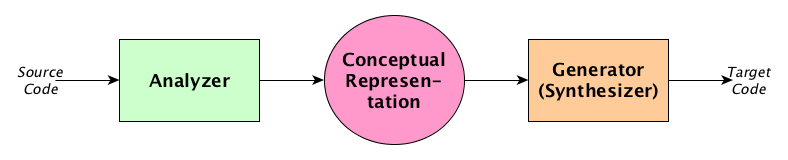
\includegraphics[scale=0.5]{images/analsyn.png}
    \caption{Arquitectura. Ray Toal, Loyola Marymount University.}
    \label{fig:compiler architecture}
\end{figure}


El desarrollo de los compiladores sigue un esquema conocido como “Teoría de Compiladores” el cual tiene su raíz junto con el nacimiento de la computación misma y más precisamente con los primeros lenguajes de programación de alto nivel. Esta teoría ha sido consolidada por varios autores\cite{aho1990compiladores}\cite{srikant2002compiler}\cite{slonneger1995formal}\cite{aho1990compiladores}\cite{meduna2007elements}\cite{appel2004modern}\cite{morgan1998building}\cite{terry1997compilers}\cite{grune2012modern}\cite{tremblay1985theory}\cite{lee1974anatomy}\cite{cooper2011engineering}\cite{gupta2010compiler}\cite{reps2007program}\cite{mak2011writing}\cite{midkiff2012automatic}\cite{seidl2012compiler}\cite{srikant2002compiler}\cite{su2011principles}\cite{mogensen2017introduction} y con el surgimiento de nuevos lenguajes de programación\cite{dasnois2011haxe}\cite{mccurdy2015haxe}\cite{klabnik2018rust}\cite{matzinger2019hands}\cite{sharma2019mastering}\cite{donovan2015go}\cite{summerfield2012programming}\cite{guney2018hands}\cite{skeen2018kotlin}\cite{adelekan2018kotlin}\cite{yousefkotlin} contínuamente está siendo puesta a prueba sin que esto haya significado modificaciones esenciales en el esquema. El caso del lenguaje Rust, de la fundación Mozilla\cite{mozillarustdoc} cuyo compilador se encuentra documentado\cite{mozillarustcdoc} en los términos de la Teoría de Compiladores, es una prueba fehaciente que las nuevas construcciones sintácticas y semánticas sobre seguridad de memoria, closures y paralelización pueden ser soportadas sin problemas por dicha teoría.

Ambas etapas están compuestas de fases internas que serán descritas en las siguientes secciones.

\subsubsection{Componentes}
A continuación brevemente se describen los componentes para un compilador que genera lenguaje ensamblador. En casos en los que los compiladores están diseñados para lenguajes de más alto nivel, o hacia máquinas virtuales, algunas de las etapas descritas son obviadas.

\begin{figure}[h]
    \centering
    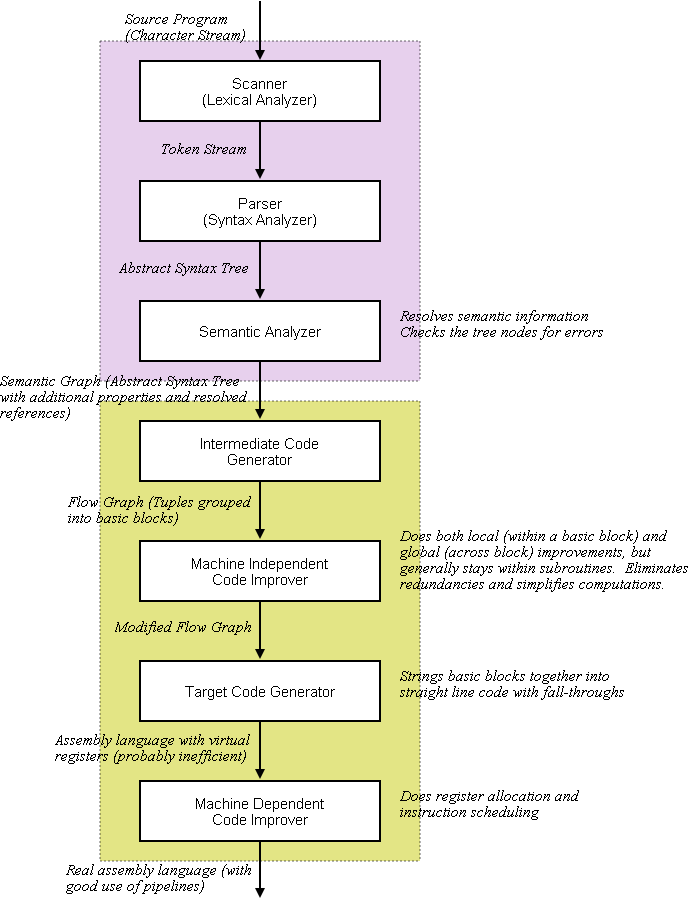
\includegraphics[scale=0.3]{images/compilerphases.png}
    \caption{Componentes de un compilador. Ray Toal, Loyola Marymount University.}
    \label{fig:compiler phases}
\end{figure}


\subsubsection{Análisis léxico (Scanner)}
El scanner convierte el flujo de caracteres correspondiente al código fuente del programa en un flujo de tokens.
Desde el código del recuadro \ref{lst:example} se puede llegar al conjunto de tokens mostrado en la Figura \ref{fig:tokens}.


\begin{lstlisting}[language=c, label={lst:example}, caption={Código de ejemplo}, captionpos={b}, frame={shadowbox}]
#define ZERO 0
unsigned  gcd (
    unsigned int x,// Algoritmo Euclideo
        unsigned y) {
            while ( /* hello */ x> ZERO) {
                unsigned temp=x;
                x=y%x;y  = temp;
            }
        return y;
}
\end{lstlisting}

\begin{figure}[h]
    \centering
    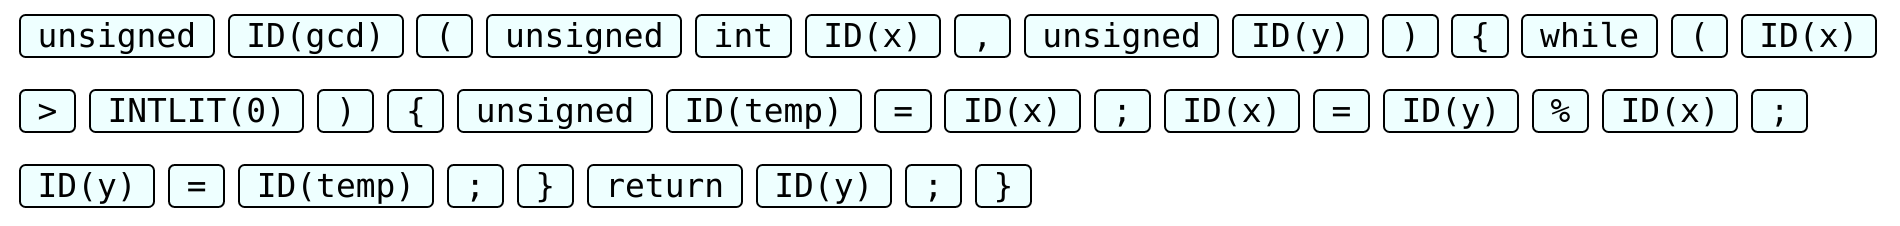
\includegraphics[scale=0.2]{images/tokens.png}
    \caption{Conjunto de tokens. Ray Toal, Loyola Marymount University.}
    \label{fig:tokens}
\end{figure}

Los escáneres se ocupan de cuestiones tales como:
\begin{itemize}
    \item Sensibilidad de mayúsculas y minúsculas (o insensibilidad)
    \item Si los espacios en blanco son significativos o no
    \item Si las nuevas líneas son significativas
    \item Si los comentarios pueden anidarse
\end{itemize}

Los errores que pueden ocurrir durante el escaneo, llamados errores léxicos, incluyen:
\begin{itemize}
    \item Encontrar caracteres que no están en el alfabeto de idioma
    \item Demasiados caracteres en una palabra o línea
    \item Un caracter no cerrado o cadena literal
    \item Un final de archivo dentro de un comentario
\end{itemize}

\subsubsection{Análisis sintáctico (Parsing)}

\begin{figure}[h]
    \centering
    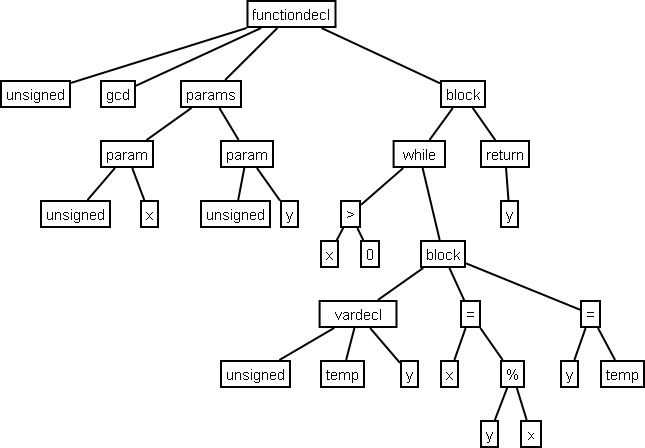
\includegraphics[scale=0.3]{images/gcdast1.png}
    \caption{Árbol sintáctico abstracto. Ray Toal, Loyola Marymount University.}
    \label{fig:ast}
\end{figure}

El árbol también puede ser guardado en forma de un string (cadena de caracteres) como es mostrado en el recuadro \ref{lst:string}

\begin{lstlisting}[label={lst:ast}, caption={AST}, captionpos={b}, frame={shadowbox}]
(fundecl unsigned gcd
  (params (param unsigned x) (param unsigned y))
  (block
    (while
      (> x 0)
      (block (vardecl unsigned temp y) (= x (% y x)) (= y temp)))
    (return y)))
\end{lstlisting}

Técnicamente, cada nodo en el AST se almacena como un objeto con campos con nombre, muchos de cuyos valores son nodos en el árbol. Hay que tener en cuenta que en esta etapa de la compilación, el árbol es definitivamente solo un árbol como se ve en la Figura \ref{fig:ast objects}. No hay ciclos.

\begin{figure}[h]
    \centering
    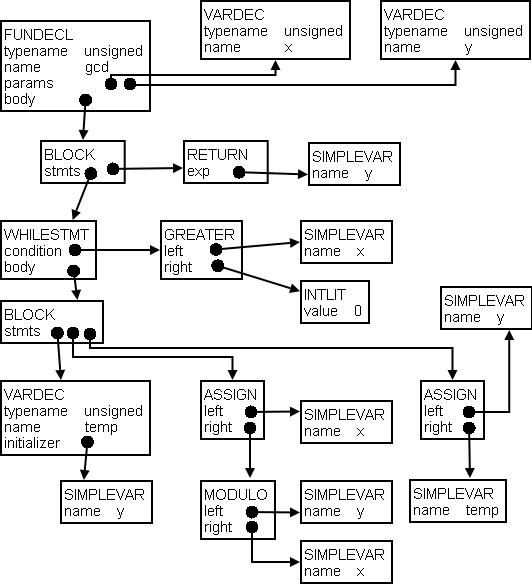
\includegraphics[scale=0.3]{images/gcdast2.png}
    \caption{Vista de objetos del AST. Ray Toal, Loyola Marymount University.}
    \label{fig:ast objects}
\end{figure}

Los errores que pueden ocurrir durante el análisis, llamados errores de sintaxis incluyen cosas como las siguientes, en C:

\begin{itemize}
    \item \texttt{42 = x * 3}
    \item \texttt{i = /5}
    \item \texttt{j = 4 * (6 - x;}
\end{itemize}


\subsubsection{Análisis semántico}
Durante el análisis semántico se deben verificar las reglas de legalidad y, al hacerlo, atar las piezas del árbol de sintaxis (resolviendo las referencias de los identificadores, insertando operaciones de conversión para coerciones implícitas, etc.) para formar un gráfico semántico.

Continuando con el ejemplo anterior, el AST se puede apreciar como en la Figura \ref{fig:ast semantic}.

\begin{figure}[h]
    \centering
    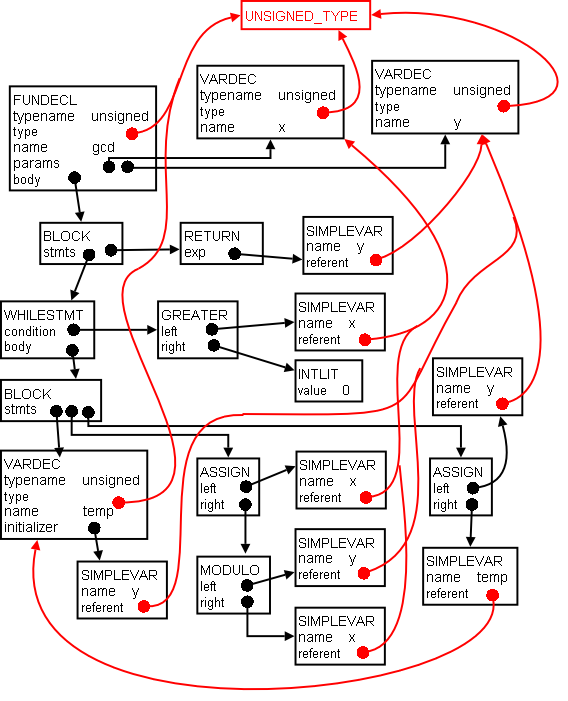
\includegraphics[scale=0.3]{images/gcdsemgraph.png}
    \caption{AST con análisis semántico. Ray Toal, Loyola Marymount University.}
    \label{fig:ast semantic}
\end{figure}

Obviamente, el conjunto de reglas permitidas es diferente para cada idioma. Los ejemplos de que se pueden ver en un lenguaje similar a Java incluyen:
\begin{itemize}
    \item Múltiples declaraciones de una variable dentro de un ámbito.
    \item Referencia a una variable antes de su declaración.
    \item Referencia a un identificador que no tiene declaración.
    \item Violar las reglas de acceso (público, privado, protegido, ...).
    \item Demasiados argumentos en una llamada de método.
    \item No hay suficientes argumentos en una llamada de método.
    \item Tipo de desajustes (hay toneladas de estos).
\end{itemize}

\subsubsection{Generación de código intermedia}
El generador de código intermedio produce un gráfico de flujo formado por \textit{tuplas} agrupadas en bloques básicos. Para el ejemplo anterior, se ve en la Figura \ref{fig:flowchart intermediate}.

\begin{figure}[h]
    \centering
    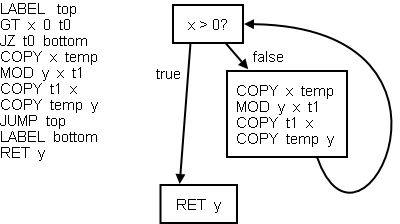
\includegraphics[scale=0.3]{images/gcdflowgraph.png}
    \caption{Gráfico de flujo intermedio. Ray Toal, Loyola Marymount University.}
    \label{fig:flowchart intermediate}
\end{figure}

\subsubsection{Mejoras de código independientes de la arquitectura}
La mejora de código que se realiza en el gráfico semántico o en el código intermedio se denomina optimización de código independiente de la arquitectura. En la práctica hay una gran cantidad de optimizaciones conocidas\cite{srikant2018compiler}\cite{emmanuel2017newtrends} (mejoras), pero ninguna realmente se aplica a nuestro ejemplo de ejecución.

\subsubsection{Generación de código}
No se pretende que el lector interprete el assembler, sino que se aprecie que mediante una optimización la lógica del programa se mantiene y su salida es más pequeña.

La generación de código produce el código de destino real, o algo cercano. Esto es lo que se obtiene al ensamblar con gcc 6.3 orientado a x86-64, sin ninguna optimización.

\begin{lstlisting}[language={[x86masm]Assembler}, label={lst:assembler simple}, caption={Ejemplo assembler sin mejora}, captionpos={b}, frame={shadowbox}]
gcd(unsigned int, unsigned int):
    pushq   %rbp
    movq    %rsp, %rbp
    movl    %edi, -20(%rbp)
    movl    %esi, -24(%rbp)
.L3:
    cmpl    $0, -20(%rbp)
    je      .L2
    movl    -20(%rbp), %eax
    movl    %eax, -4(%rbp)
    movl    -24(%rbp), %eax
    movl    $0, %edx
    divl    -20(%rbp)
    movl    %edx, -20(%rbp)
    movl    -4(%rbp), %eax
    movl    %eax, -24(%rbp)
    jmp     .L3
.L2:
    movl    -24(%rbp), %eax
    popq    %rbp
    ret
\end{lstlisting}


\subsection{Mejora de código dependiente de la arquitectura}

Por lo general, la fase final en la compilación es limpiar y mejorar el código objetivo. Para el ejemplo anterior, se obtiene lo siguiente al configurar el nivel de optimización en -O3:
\begin{lstlisting}[language={[x86masm]Assembler}, label={lst:assembler improved}, caption={Ejemplo assembler con mejora}, captionpos={b}, frame={shadowbox}]

gcd(unsigned int, unsigned int):

        testl   %edi, %edi
        movl    %esi, %eax
        jne     .L3
        jmp     .L7
.L5:
        movl    %edx, %edi
.L3:
        xorl    %edx, %edx
        divl    %edi
        movl    %edi, %eax
        testl   %edx, %edx
        jne     .L5
.L1:
        movl    %edi, %eax
        Ret
.L7:
        movl    %esi, %edi
        jmp     .L1
\end{lstlisting}


\section{¿Por qué compiladores?}
Siempre se pone el foco y la responsabilidad del lado del lenguaje en el que los desarrolladores programan, pero más allá de testear, se está totalmente confiando en que el compilador que se utiliza no posea fallas de seguridad, y que como mínimo no vaya a introducir nuevas en el código desarrollado.


La seguridad informática es un desafío bastante amplio impuesto sobre el sistema. Sólo se necesita una parte que sea insegura y todo el sistema se vuelve inseguro. Sería muy dificultoso para un compilador corregir automáticamente código inseguro, ya que para ello, debería tener en su concepción una gran cantidad de aspectos pragmáticos aún no conocidos en el momento de su construcción. Pero más allá de lo anterior, el compilador está colocado perfectamente en una posición que permite ayudar a un programador o ingeniero de software a escribir sistemas seguros. La razón es porque el compilador es el único programa que tiene la posibilidad de mirar (casi) todas las líneas de un software. Obviamente lenguajes compilados como C/C++ pasan por un compilador, pero lenguajes semi-interpretados como Java también tienen un compilador para generar su bytecode e incluso código assembler es típicamente pre-procesado por el compilador. Las únicas excepciones podrían ser los lenguajes puramente interpretados, con algunos otras casos muy particulares\cite{secenhancedcompilers}, aunque la interpretación puede verse como una suerte de compilación en línea, compilación bajo demanda o compilación JIT (\textit{Just in Time})\cite{bolc2012design}\cite{mak2011writing}.

\textit{¿Hasta dónde debería uno confiar que una declaración en un programa está libre de Caballos de Troya? Tal vez es más importante confiar en las personas que desarrollaron el software directamente.}

Lo describe claramente Ken Thompson, desde 1984 en su artículo \textbf{Reflections on trusting trust} (reflecciones en confiar en la confianza):
\begin{displayquote}
    \textit{"La moral es obvia. No podés confiar en un código que no creaste en su totalidad. (Especialmente el código de compañías que emplean a personas como yo). Ninguna verificación o escrutinio a nivel de fuente te protegerá de usar código no confiable. Al demostrar la posibilidad de este tipo de ataque, elegí el compilador de C. Podría haber elegido cualquier programa de manejo de software, como un ensamblador, un cargador o incluso un microcódigo de hardware. A medida que el nivel del programa disminuye, estos errores serán cada vez más difíciles de detectar. Un bug de microcódigo bien instalado será casi imposible de detectar."}
    \newline{\null\hfill -- Ken Thompson}
\end{displayquote}

El "ataque" del cual habla está separado en dos etapas, y consta de cómo hipotéticamente modifica un compilador para generar backdoors (puertas traseras). En la primera etapa, el código en C contiene código visiblemente obvio para modificar la lógica dado un patrón determinado, de un programa de acceso, y como bien dice:
\textit{Tal descarado código no pasaría desapercibido por mucho tiempo. Incluso la lectura más casual del código fuente del compilador de C levantaría sospechas.}

En la segunda etapa es donde la modificación de un compilador con fines maliciosos se pone interesante. En adición a agregar código al compilador de C para corromper un programa en particular también agrega código al compilador para corromperse a sí mismo. Es decir, que si se compilara con ese compilador maligno otro compilador en base a un código limpio, se agregaría la lógica necesaria al nuevo compilador para que cada vez que procese un software de acceso le inserte un \textit{backdoor}.

No necesariamente tiene que ser con intenciones malignas, así como hay errores de seguridad en la mayoría de los programas, un compilador no está exento a esto, y las mismas fallas podrían generar comportamientos inesperados en la compilación.


\subsection{Optimizaciones y comportamiento inesperado}
Investigadores del laboratorio de Ciencias de la computación e inteligencia artificial del MIT publicaron un paper (\textit{Towards Optimization-Safe Systems: Analyzing the Impact of Undefined Behavior}) analizando el problema optimización de código inestable, el cual es código que el compilador quita porque incluye comportamiento indefinido. Dicho código es el que puede comportarse de maneras inesperadas, como dividir por cero, una desreferencia de puntero nulo y \textit{buffer overflows} (rebalse de búferes).

A diferencia de otro código, los desarrolladores de compiladores son libres de decidir cómo lidiar con este tipo de comportamientos. En algunos casos eligen eliminar ese código completamente, lo cual puede llevar a vulnerabilidades si el código en cuestión posee chequeos de seguridad.

Estos investigadores estudiaron una docena de compiladores C/C++ más comúnmente utilizados para observar cómo lidian con código indefinido. Encontraron que, con el tiempo, los compiladores están poniéndose más agresivos en cómo lidian con ese código, usualmente sólo quitándolo, incluso por defecto o en pequeños niveles de optimización. Ya que C/C++ es bastante liberal respecto a permitir comportamiento indefinido, es más susceptible a errores y amenazas de seguridad como resultado de código inestable.

Tanto es el hecho que existe una categoría de seguridad específicamente para estos casos, llamada \textit{optimización insegura de compilación}. A continuación un ejemplo.\cite{insecureoptOWASP}

\begin{lstlisting}[language={c}, label={lst:vulnerable code}, caption={Código vulnerable}, captionpos={b}, frame={shadowbox}]
void GetData(char *MFAddr) {
    char pwd[64];
    if (GetPasswordFromUser(pwd, sizeof(pwd))) 
     if (ConnectToMainframe(MFAddr, pwd)) {
             // Interaction with mainframe
        }
      }
      memset(pwd, 0, sizeof(pwd));
}
\end{lstlisting}

El código en el ejemplo del cuadro \ref{lst:vulnerable code} se comportaría correctamente si se ejecutara de manera literal, pero si el código se compila utilizando la opción general de optimización, como las de los compiladores de C++ Microsoft Visual C ++ ® .NET o GCC 3.x, la llamada a memset() se eliminará como un almacenamiento inactivo porque el búfer \textit{pwd} no se usa después de que su valor se sobrescribe. Debido a que el búfer pwd contiene un valor sensible, la aplicación puede ser vulnerable a un ataque si los datos se quedan en la memoria. Si los atacantes pueden acceder a la región correcta de la memoria, pueden usar la contraseña recuperada para obtener el control del sistema.\cite{wikiseicmuedu}
 
Otro ejemplo más impactante que terminó afectando a muchos sistemas Linux/GNU, fue un error introducido en el kernel debido a una optimización.
Si bien los detalles técnicos sobre esto son un poco complejos, en general, lo que sucede puede explicarse fácilmente. El código vulnerable se encuentra en la implementación de una librería. Básicamente, lo que sucede aquí es que el desarrollador inicializó una variable (\textbf{sk} en el fragmento de código a continuación) a un cierto valor que puede ser \textit{NULL}. El desarrollador verificó correctamente el valor de esta nueva variable par de líneas más tarde y, si es 0 (\textit{NULL}), simplemente devuelve un error. El código se ve así:\cite{iscsansedukernelvuln}

\begin{lstlisting}[language={c}, label={lst:kernel vuln}, caption={Código vulnerable 2}, captionpos={b}, frame={shadowbox}]
struct sock *sk = tun->sk;  // initialize sk with tun->sk
...
if (!tun)
    return POLLERR;  // if tun is NULL return error
\end{lstlisting}

Este código se ve perfectamente bien, y lo es, al menos hasta que el compilador toma esto en sus manos. Mientras optimiza el código, verá que la variable ya ha sido asignada y eliminará el bloque \textit{if} (la comprobación si \textit{tun} es NULL) completamente del código compilado resultante. En otras palabras, el compilador introducirá la vulnerabilidad al código binario, que no existía en el código fuente. Esto hará que el kernel intente leer / escribir datos desde la dirección de memoria \textit{0x00000000}, que el atacante puede \textit{mapear} a la zona de usuario, controlando el flujo de ejecución. 

\textbf{Vulnerabilidades en intérpretes}

Los intérpretes no son el foco de discusión en esta investigación, pero el contenido aplica de igualmente manera a ellos también.

Todas las vulnerabilidades alguna vez reportadas tienen asignado un identificador único llamado CVE (Common Vulnerability Enumeration). En el sitio oficial de la lista se puede encontrar que intérpretes como Ruby\cite{rubyvulns}, Python\cite{pythonvulns} y PHP\cite{phpvulns} poseen 13, 45 y 599 vulnerabilidades reportadas hasta el momento de esta redacción.


\section{Tecnologías blockchain}
En esta sección se enumeran tecnologías cuya estructura principal es del tipo blockchain, con las que se trabajó en esta tesis y forman parte de las principales razones por la que fue impulsada esta investigación, dada la popularidad que han obtenido en los últimos años.


\subsection{Bitcoin}
La idea de tener una moneda digital no es nueva. Antes de las \textit{cryptocurrencies} (criptomonedas), existieron muchos intentos de crear una. El principal desafío que la mayoría encontraba era solucionar el problema de \textit{double spend} (doble gasto). Un bien digital tiene que de alguna manera ser utilizado sólo una vez para prevenir que se copie y efectivamente falsifique.\cite{briefhistorycryptoledger}

Diez años antes de las \textit{cryptocurrencies}, el concepto había sido introducido por un ingeniero en computación llamado Wei Dai. En 1998, publicó un paper donde discutió una propuesta llamada \textit{B-money}. Discutió la idea de una moneda digital, que podía ser enviada junto con un grupo de pseudónimos irrastreables. Ese mismo año, otro intento bajo el nombre \textit{Bit Gold} fue escrito por Nick Szabo. Bit Gold incluyó la posibilidad de crear una moneda digital descentralizada. La idea de Szabo fue motivada por las ineficiencias que se encuentran hoy en día en el sistema financiero tradicional (FIAT), como requerir metales para construir monedas, y para reducir la cantidad de confianza que hay que tener para realizar transacciones. Si bien ambos proyectos nunca fueron oficialmente ejecutados, fueron parte de la inspiración de \textit{Bitcoin}\cite{narayanan2016bitcoin}.

En el 2008 Satoshi Nakamoto publicó un artículo (\textit{white paper}) llamado \textit{Bitcoin: A Peer-to-Peer Electronic Cash System}, describiendo la funcionalidad de la red blockchain de Bitcoin: \textit{una red sin permiso tolerante a fallos bizantinos} (resistencia de un sistema informático tolerante a faltas) \textit{criptográficamente segura}.

\begin{displayquote}
    \textit{"Mucha gente descarta automáticamente las e-currency como una causa perdida por todas las compañías que fallaron hacerlo desde 1990. Espero que sea obvio que lo que las llevó a la perdición fue su naturaleza de tener un sistema central controlado. Creo que esta es la primera vez que estamos intentando un sistema descentralizado, no basado en la confianza."}
    \newline{\null\hfill -- Satoshi Nakamoto.}
\end{displayquote}

\subsection{Estructura blockchain}
La blockchain es un libro de registro distribuido punto a punto, seguro, y se utiliza para registrar transacciones. El contenido del registro solo se puede actualizar agregando otro bloque vinculado al anterior. También se puede ver como una plataforma donde las personas pueden realizar transacciones de todo tipo sin la necesidad de un árbitro central o de confianza.

\textit{La base de datos creada se comparte entre los participantes de la red de manera transparente, por lo que todos pueden acceder a su contenidos. La gestión de la base de datos se realiza de forma autónoma utilizando redes punto a punto y un servidor de timestamping, es decir que permite demostrar que una serie de datos han existido y no han sido alterados desde un instante específico en el tiempo. Cada bloque en una blockchain está organizado de tal manera que hace referencia al contenido del bloque anterior.}\cite{101blockchains}

\textit{Los bloques que forman una blockchain contienen lotes de transacciones validadas por los participantes en una red. Cada bloque viene con un hash criptográfico de un bloque anterior en la cadena.}\cite{101blockchains}

\begin{notesBox}
    Bitcoin y Blockchain no son sinónimos. Blockchain es la estructura que Bitcoin posee como base para impulsar sus aplicaciones.
\end{notesBox}


\subsection{Smart Contracts}
Un smart contract es un código de computadora corriendo sobre una blockchain que posee un conjunto de reglas bajo las cuales las partes de ese contrato acceden para interactuar uno con el otro. Si-y-cuando esas reglas se cumplan, el acuerdo es automáticamente impuesto. El código del smart contract facilita, verifica, y hace cumplir la negociación o performance de un acuerdo o transacción. Es la forma más simple de automatización descentralizada.

Es un mecanismo que envuelve bienes digitales de dos o más partes, donde algunas o todas las partes depositan bienes en el contrato y los bienes son automáticamente redistribuidos entre esas partes dependiendo de una fórmula basada en determinados datos, que no son conocidos al momento de la iniciación del contrato. 

El término se presta a confusiones porque un smart contract no es inteligente, ni debería ser confundido con un contrato legal:
\begin{itemize}
    \item Un smart contract es tan inteligente como las personas que lo programaron con la información que tenían disponible en ese momento.
    \item Mientras que tienen el potencial de poder ser contratos legales no deben confundirse con contratos legales aceptados por las cortes y la ley. Sin embargo, probablemente se vaya a ver una fusión de estos dos en el futuro.
\end{itemize}

Si bien la descripción anterior es acertada, y una definición que se puede observar en muchas fuentes, el autor cree que es demasiada específica. Un smart contract es algo más abstracto.

Entonces, se puede resaltar lo más importante de la siguiente manera: son auto verificables, auto ejecutables y resistentes a la manipulación; pueden transformar responsabilidades legales en procesos automatizados, garantizar un gran grado de seguridad, reducen la dependencia de intermediarios confiables y poseen costos de transacción bajos. 


\subsection{Ethereum}
En el 2013 un jóven llamado Vitalik Buterin\cite{miethereumvitalik}, co-fundador de la Bitcoin Magazine propuso \textbf{Ethereum} en un paper llamado \textit{‘Ethereum: A Next-Generation Smart Contract and Decentralized Application Platform’}. Preocupado por las limitaciones de Bitcoin, comenzó a trabajar en lo que él pensaba que sería una blockchain maleable que pueda realizar varias funciones además de ser una red punto a punto. Ethereum\cite{101blockchainseth} nació como una nueva blockchain pública con funcionalidades adicionales, en comparación con Bitcoin.

\begin{displayquote}
\textit{"Bitcoin es excelente como dinero digital, pero su lenguaje de scripting es demasiado débil para que se puedan construir aplicaciones avanzadas de forma seria."}
\newline{\null\hfill -- Vitalik Buterin}
\end{displayquote}

Lanzado oficialmente en 2015, Ethereum ha evolucionado hasta convertirse en una de las aplicaciones más grandes de la tecnología de blockchain, dada su capacidad para respaldar los \textit{smart contracts} utilizados para desarrollar aplicaciones descentralizadas. La plataforma ha logrado reunir una comunidad activa de desarrolladores que la han visto convertirse en un verdadero ecosistema.

Procesa la mayor cantidad de transacciones diarias gracias a su capacidad para soportar contratos inteligentes y aplicaciones descentralizadas. Su capitalización de mercado también se ha incrementado significativamente en el espacio de las criptomonedas.

En la Figura \ref{fig:blockchain history} se muestra una cronología para repasar visualmente el proceso.

\begin{figure}[h]
    \centering
    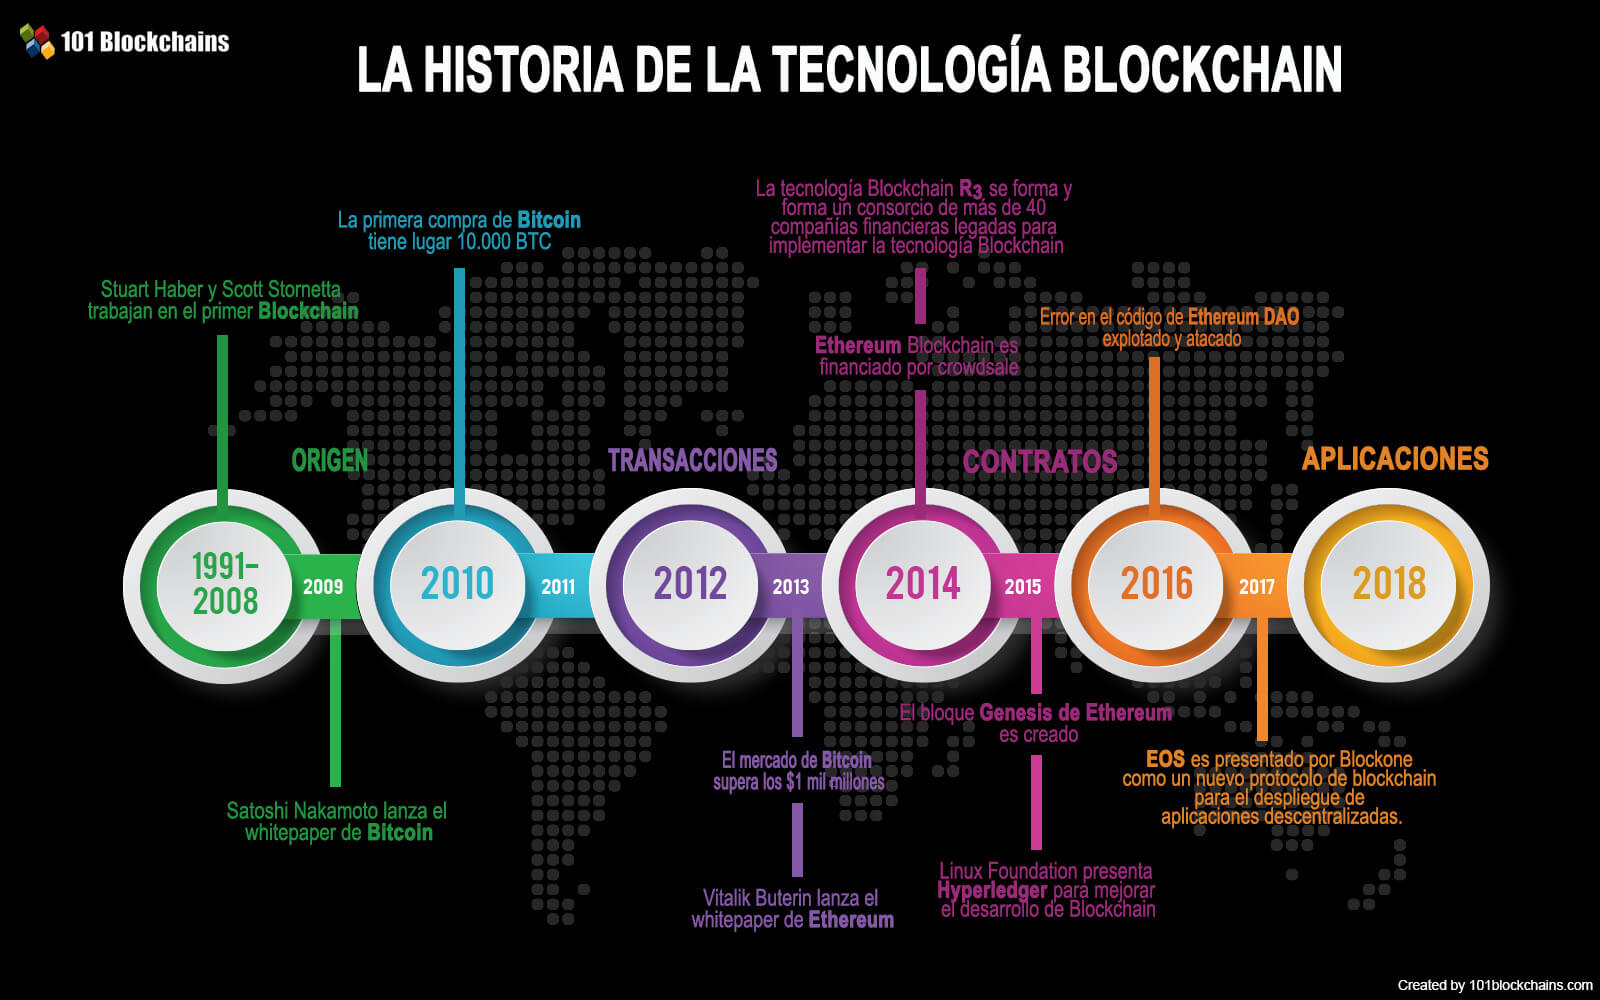
\includegraphics[scale=0.3]{images/historiablockchain.jpg}
    \caption{ Cronología de tecnologías blockchain por 101blockchains.}
    \label{fig:blockchain history}
\end{figure}

\subsection{Ethereum Virtual Machine}
La Ethereum Virtual Machine (\textbf{EVM}) es el contexto en el cual los smart contracts de la red de Ethereum viven y se ejecutan. Posee un stack de registros de 256 bits, diseñada para correr el código exactamente como fue desarrollado. Es el mecanismo de consenso fundamental para Ethereum. La definición formal de la EVM está especificada en el Ethereum Yellow Paper.

\begin{figure}[h]
    \centering
    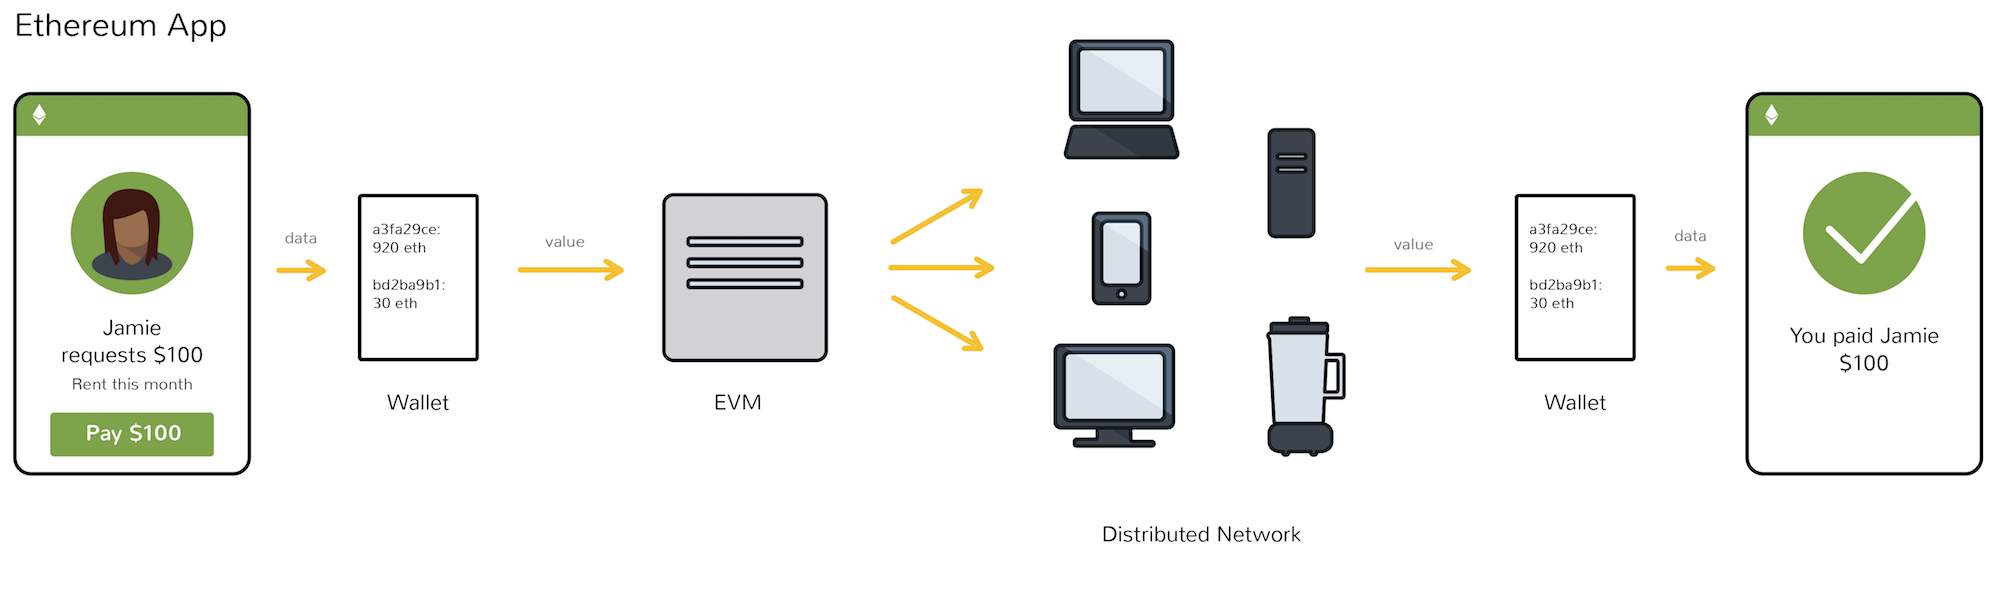
\includegraphics[scale=0.5]{images/ethflowapp.png}
    \caption{Diagrama de despliege, por Coindesk.}
    \label{fig:ethereum app}
\end{figure}

\subsection{¿Cómo es Ethereum diferente a Bitcoin?}
Si bien hay varias similitudes entre Ethereum y Bitcoin, también hay diferencias significativas:
\begin{enumerate}
    \item Bitcoin opera sólo como cryptocurrency, mientras que Ethereum ofrece diversos métodos de interacción, incluyendo cryptocurrency (Ether), smart contracts y la Ethereum Virtual Machine.
    \item Están basados en distintos protocolos de seguridad: Ethereum eventualmente utilizará un sistema \textit{proof of stake} (PoS) en contraposición al sistema \textit{proof of work} (PoW) utilizado por Bitcoin, aunque en este momento utilizan el mismo hasta que el cambio suceda. \textit{Explicar las diferencias y alcances de PoS vs PoW escapa del contexto de la investigación.}
    \item El tiempo promedio de generación de un bloque en Ethereum es de 12 segundos contra 10 minutos de Bitcoin. Esto se traduce a más confirmaciones de bloque, lo que permite a los mineros de Ethereum a completar más bloques y recibir más Ethers.
    \item Ethereum usa un sistema de cuentas en donde los valores en Wei (mínima unidad de representación de un Ether, \verb|1x10^18|) son debitados de una cuenta hacia otra, al contrario del sistema de UTXO (\textit{Unspent Transaction Output}) de Bitcoin, que es más análogo a gastar dinero y recibir cambio. Ver Figura \ref{fig:ethereum state transaction}.
    \item Ethereum posee una máquina virtual que permite escribir smart contracts con un lenguaje bytecode \textit{turing completo}.
    \item La moneda de Bitcoin se representa mediante la sigla BTC, y la de Ethereum mediante ETH.
\end{enumerate}

\begin{figure}[h]
    \centering
    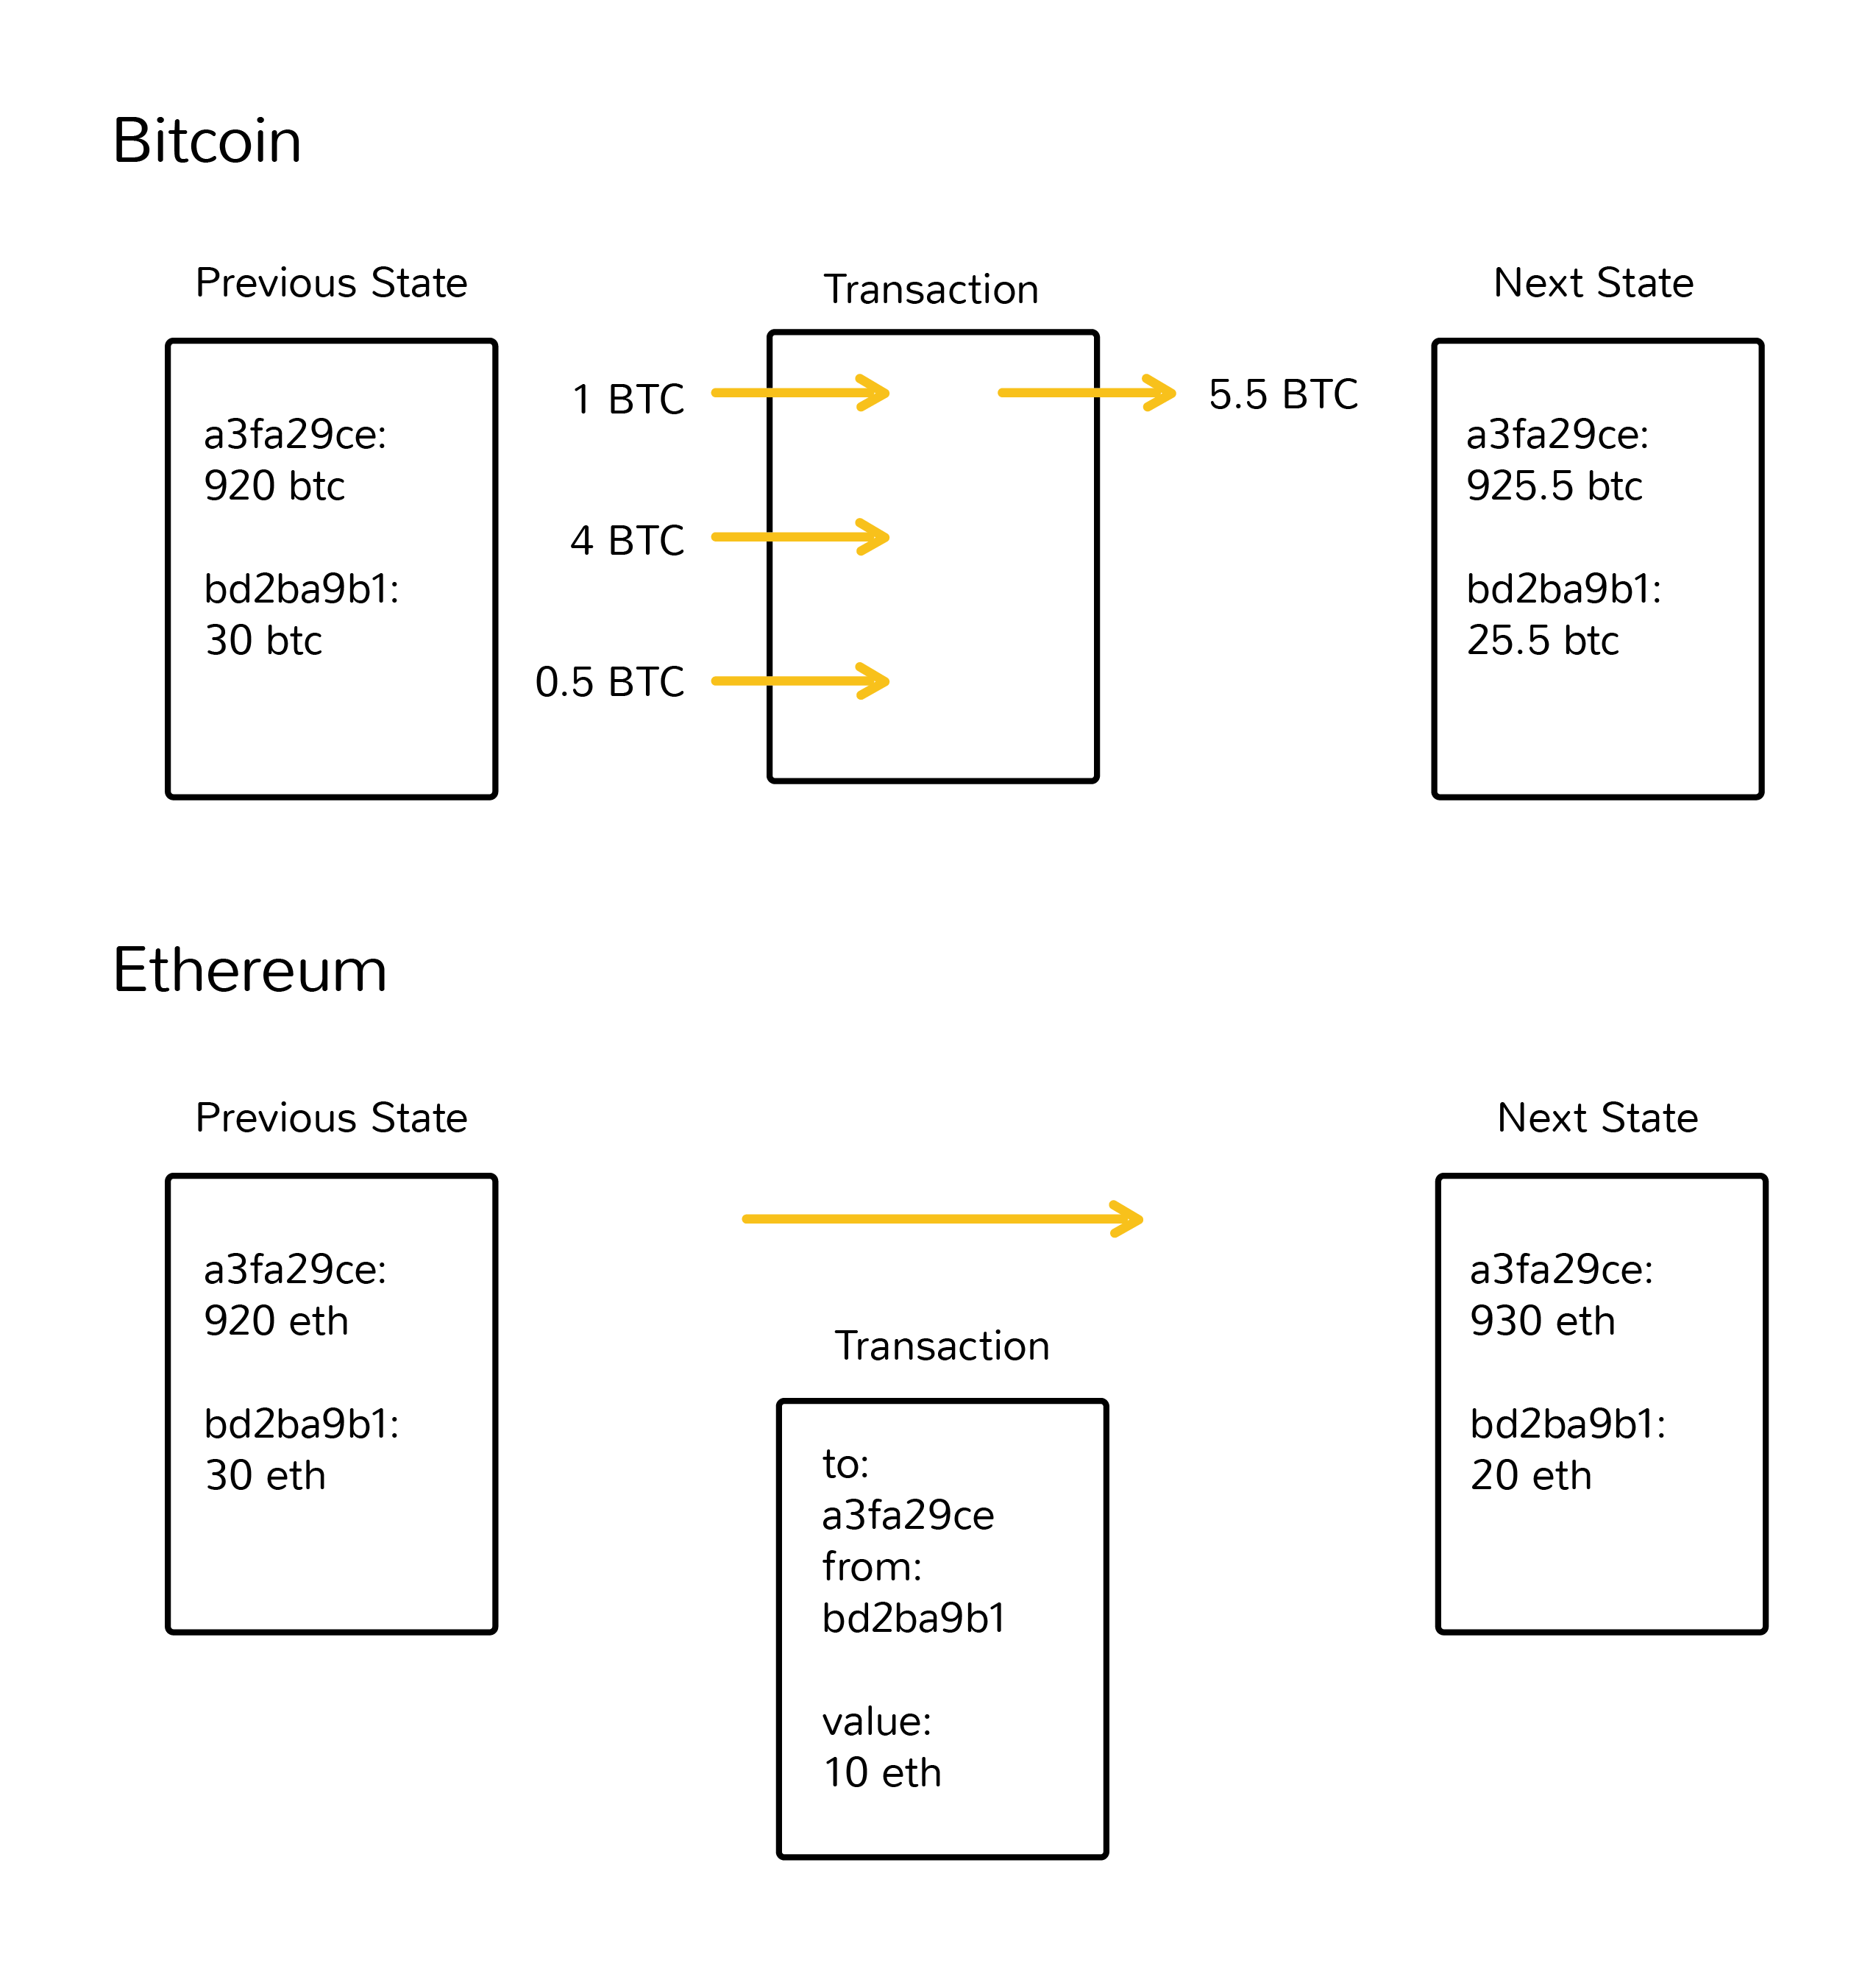
\includegraphics[scale=0.5]{images/statecoindesk.png}
    \caption{Diferencia del estado de las transacciones por Coindesk.}
    \label{fig:ethereum state transaction}
\end{figure}


\subsection{Lenguajes de programación para la EVM}
Los smart contracts de Ethereum pueden ser escritos en \textbf{Solidity}\cite{soliditylink} (un lenguaje de bibliotecas que posee similitudes con C y JavaScript), \textbf{Serpent}\cite{serpentlink} (similar a Python, pero deprecado), \textbf{LLL}\cite{llllink} (un lenguaje bajo nivel similar a Lisp), \textbf{Mutan}\cite{mutanlink} (basado en Go, pero también deprecado), \textbf{Vyper}\cite{vyperlink} (orientado a la investigación, fuertemente tipado, basado en Python, recursivo), y recientemente la empresa \textbf{BlockStack}\cite{blockstacklink} presentó \textbf{Clarity}\cite{claritylink} (tiene intencionado optimizar la predictibilidad y la seguridad).

Esto convierte a Solidity en el lenguaje más utilizado, o de facto, a la hora de desarrollar smart contracts en \textbf{Ethereum Network}\cite{ethereumhowlink}.


\section{Auditando blockchains}
Entonces, repasando un poco ahora que se posee la terminología necesaria: se puede desarrollar un smart contract en Solidity, que es compilado a bytecode, y si todo es correcto, será puesto en funcionamiento (\textit{deployado}) de manera inmutable a la blockchain. Allí todos los nodos que poseen máquinas virtuales tendrán una copia de ese contrato, y de ahora en más deberán llegar a un consenso en cuanto a si los interacciones que lo involucran y sus modificaciones de estado son correctos.

Entendiendo esto, se pueden definir las siguientes maneras de auditar una tecnología blockchain que utiliza smart contracts:
\begin{itemize}
    \item \textbf{Análisis estático al código}\newline
    Análisis al código mediante la automatización de herramientas que buscan patrones comunes susceptibles a errores y fallas de seguridad.
    \item \textbf{Análisis dinámico del contrato}\newline
    Analizar mediante cualquier medio el comportamiento del contrato, interactuando en vivo en la blockchain. Generalmente se replica en un entorno seguro, como en una red de testeo, conocidas como testnets.
    \item \textbf{Ingeniería inversa al bytecode deployado}\newline
    Analizar directamente el código resultante de la compilación, es decir el bytecode, lenguaje que interpreta la EVM. Generalmente se utiliza para observar si se introdujeron errores en el proceso de deployment, o para los contratos cuyo código fuente no se posee.
    \item \textbf{Verificación formal}\newline
    Es el mecanismo mediante el cual se prueba la correctitud de un contrato, basada en la verificación formal de lo que se supone que debería hacer. Una manera de realizar análisis estático pero sumamente compleja. Generalmente lo realiza quién lo desarrolla.
    \item \textbf{Ejecución simbólica}\newline
    Mecanismo para analizar un contrato con el fin de entender qué entradas estimulan qué partes de él.
\end{itemize}

Algunas de estas técnicas implican analizar directamente el bytecode como output del compilador de Solidity por ejemplo, o el bytecode del contrato deployado en la blockchain, por más que se posea el fuente.

¿Por qué se ofrece esta alternativa? Porque es lógico asumir luego de las declaraciones anteriores, que no se puede confiar en la manera en la que los compiladores optimizan o interpretan el código. Por eso es necesario comprobar que la salida interpretada por la EVM tiene de hecho la intención con la que fue diseñado.

\section{¿Por qué el compilador de Solidity?}
En el momento de la escritura de esta sección, la moneda que maneja la Ethereum Network ether, es decir 1 \textbf{ETH}, equivale a un total de \textbf{US\$}266.29. El volúmen de transacciones de ETH en dólares de las últimas 24 horas es de \textbf{US\$}8.584.415.157 o 939.202 BTC. Es decir, con la cotización del dólar en Argentina, equivale a un total de \textbf{AR\$}372.282.118.457,18\cite{coinmarketcap}
El \textbf{ether} no es el único bien que posee muchas transacciones diarias. También existen los tokens, que se pueden comprar con monedas. Una moneda opera independientemente, mientras que un token posee un uso específico en el ecosistema de un proyecto. Son creadas sobre la red de Ethereum, gestionadas mediante smart contracts. Algunos ejemplos y sus volúmenes en las últimas 24 horas de esta redacción son:

\begin{itemize}
    \item Dai: DAI \$22,038,619 USD 
    \item Maker: MKR \$1,514,750 USD 
    \item OmiseGo: OMG \$119,081,815 USD 
    \item Basic Attention Token: BAT \$66,837,473 USD
    \item 0x: ZRX \$17,960,636 USD 
    \item Augur: REP \$6,113,229 USD
    \item Usd Coin Classic: USDC \$177,029,191 USD
    \item Paxos Standard Token: PAX \$128,207,385 USD
    \item Status: SNT \$16,693,466 USD
    \item Golem: GNT \$1,843,572 USD 
    \item Decentraland: MANA \$10,516,180 USD
\end{itemize}


Esto no incluye otras plataformas de Ethereum paralelas como \textbf{EOS}, \textbf{Tron}, \textbf{IOST} o más, en donde algunos de sus volúmenes en las últimas 24 horas supera los miles de millones de dólares en sólo alguna de las aplicaciones que corren, como por ejemplo \textbf{TRONBet} para Tron, \textbf{dice2.win} para ETH, o \textbf{EOSJacks} para EOS\cite{dappradar}.

El interés que ha habido en este ambiente por la cantidad de dinero que manejan ha aumentado en gran cantidad desde sus comienzos. En el sitio de Ledger, fabricantes de billeteras digitales en hardware, muestran un diagrama de tiempo\cite{ledgerhackstime} con todos los hackeos que han recibido los sitios de intercambio (\textbf{exchanges}) desde sus comienzos. Los costos en pérdidas superan el billón de dólares en costos.

\subsection{Smart contract hacks}
En esta sección se presentan tres ejemplos de \textit{hackeos} de alto impacto, de los más populares que han acontecido desde el momento en el que se empezó a interactuar con Smart Contrats en la red de Ethereum.


\subsubsection{El DAO hack}
Una \textbf{DAO} es una Organización Autónoma Descentralizada o una organización que se ejecuta a través de smart contracts. Las decisiones se toman digitalmente mediante la votación de los miembros de la organización, eliminando la necesidad de documentos y personas que gobiernan y, en consecuencia, un sistema de control descentralizado.

En este caso, la DAO comprendía una serie de contratos inteligentes destinados a democratizar cómo se financiaban los proyectos de Ethereum. Un hacker, al darse cuenta de una vulnerabilidad, robó USD\$ 3.6 millones de Ethers mediante la explotación de una función (\textit{fallback}) en el código que fue expuesto a una vulnerabilidad conocida como \textit{reentrancy} (re-entrada). Para recuperar los fondos, se tuvo que tomar una dura decisión, atentando contra la fe de los usuarios, que condujo a la creación de Ethereum Classic y Ethereum como dos cadenas separadas.\cite{daoattack}


\subsubsection{Multi-firma Wallet hack de Parity}
La empresa \textbf{Parity} hizo “billeteras” (\textit{wallets}) de software multi-firma (multi-sig) para la gestión de la criptomoneda Ether. Estas wallets multi-sig eran contratos inteligentes disponibles en una base de código abierto que requerían más de una firma digital (clave privada) antes de que el Ether asociado con ellos pudiera ser aprobado para su transferencia.
Un hacker desconocido robó 150,000 Ethers, alrededor de USD\$30.000.000 en ese momento\cite{parityheist}.

\subsubsection{Wallets de Parity congeladas por un usuario}
Apenas unos meses después del hackeo en julio de 2017, un usuario explotó accidentalmente una vulnerabilidad en el código de la biblioteca de Parity para las wallets multi-sig, congelando más de 513.774,16 ETH, lo que representaba en esa época más de USD\$106.864.992\cite{parityfreeze}.\newline

\textbf{En conclusión},\textit{ no solo se tiene la importancia de auditar un compilador por las razones mencionadas anteriormente, sino que al auditar un compilador como el de Solidity, se estaría auditando un compilador cuyo código emitido e inmutable corre en todas las máquinas virtuales de todos los nodos de una red. Es decir que si se encuentra la manera de, vulnerar los contratos para obtener su balance, o la manera de emitir un mensaje que detenga el funcionamiento de toda la red, sería catastrófico.}
